% =====================================================================================
% RAPORT KOŃCOWY — QEM / KN Axion, Politechnika Wrocławska
% Główna teza: routing wstrzykuje błąd KOHERENTNY -> łamie liniowość CDR
%   -> załamanie jest TOPOLOGICZNIE OGÓLNE -> circuit twirling to naprawia,
%      a zysk ROŚNIE z budżetem bramek dwukubitowych.
% Status: wszystkie sekcje rozpisane; [CZEKA w3] = do aktualizacji po 3. oknie driftu.
% =====================================================================================
\documentclass[11pt]{article}
\usepackage[margin=2.5cm]{geometry}
\usepackage[T1]{fontenc}
\usepackage[utf8]{inputenc}
\usepackage[polish]{babel}
\usepackage{amsmath,amssymb,graphicx,booktabs,hyperref,siunitx}
\usepackage[dvipsnames]{xcolor}
\usepackage{tikz}
\usetikzlibrary{positioning,decorations.pathreplacing}
\hypersetup{colorlinks=true, linkcolor=NavyBlue, citecolor=NavyBlue, urlcolor=NavyBlue,
            linktoc=all, pdfborder={0 0 0}}
\newcommand{\todo}[1]{\textcolor{red}{[\textbf{TODO:} #1]}}
\newcommand{\expv}{\langle O\rangle}

\begin{document}

% ===================== STRONA TYTUŁOWA =====================
\begin{titlepage}
\centering
\vspace*{3cm}

{\LARGE\bfseries Przeprowadzenie topology-aware ewaluacji wpływu narzutu SWAP
i~rozmieszczenia kubitów na skuteczność mitygacji błędów oraz kodowania logicznego
na sprzęcie nadprzewodzącym\par}


\vspace{3cm}
{\Large Karina Leskiewicz\par}
\vspace{0.4cm}


\vfill
{\large \today\par}
\end{titlepage}

% ===================== SPIS TREŚCI =====================
\tableofcontents
\newpage

\begin{abstract}
Komputery kwantowe ery NISQ dysponują dziś dziesiątkami kubitów o~wierności bramek dwukubitowych
rzędu $99\%$. Pełna korekcja błędów pozostaje poza zasięgiem, ponieważ wymaga zakodowania jednego
kubita logicznego w~setkach lub tysiącach kubitów fizycznych. Aby uzyskiwać wyniki
\emph{teraz}, trzeba radzić sobie z~nieskorygowanym szumem, a~jedynym praktycznym narzędziem jest
\emph{mitygacja} błędów (QEM). Metody mitygacji nie działają jednak bezwarunkowo: każda zakłada
określony model szumu, każda ma własny narzut pomiarowy i~każda przestaje się opłacać poza pewnym
reżimem. Praca poszukuje usystematyzowanego sposobu oceny, które metody mają szansę pomóc
w~konkretnych warunkach.

Jako zmienną porządkującą przyjęto \emph{narzut routingu}: bramki SWAP, które kompilator musi
wstawić, gdy obwód logiczny nie odwzorowuje topologii urządzenia. Ustalono
obciążenie obliczeniowe (zamrożony klasyfikator wariacyjny) i~zmieniamy wyłącznie koszt routingu,
mierząc na trzech rzeczywistych procesorach nadprzewodzących IQM: \textbf{ODRA} (Spark, 5~kubitów,
topologia gwiazdy), \textbf{Garnet} (20~kubitów, krata) oraz \textbf{Emerald} (54~kubity, krata,
klasycznie niesymulowalny). Ten sam obwód logiczny kosztuje na nich od 12 do 114 bramek CZ.

Wyłania się z~tego usystematyzowany obraz reżimów. Trzy metody okazują się w~tym obciążeniu
bezużyteczne: mitygacja błędu odczytu (REM) zmniejsza błąd wartości oczekiwanej, lecz nie zmienia
\emph{żadnej} decyzji klasyfikatora, dynamiczne odsprzęganie (DD) pogarsza wynik w~każdym punkcie
drabiny, a~detekcja w~kodzie $[[4,2,2]]$ nie zwraca kosztu post-selekcji. Praktyczny wybór sprowadza
się do dwóch pozostałych.

Ekstrapolacja do zerowego szumu (ZNE) wygrywa poniżej punktu równowagi w~okolicy 39~bramek CZ
i~jest tam siedmiokrotnie tańsza od regresji danych Clifforda (CDR). Jej okno użyteczności jest
jednak ograniczone z~\emph{obu} stron, a~dolną krawędź tego okna wyprowadzono analitycznie
z~konstrukcji estymatora Richardsona i~potwierdzono na sprzęcie dla dwóch różnych zbiorów węzłów
ekstrapolacji, bez ani jednego parametru dopasowywanego do danych. Powyżej punktu równowagi
najlepsze wyniki daje CDR, lecz i~ona załamuje się w~sposób \emph{topologicznie ogólny}: jakość
dopasowania liniowego $r^2$ spada monotonicznie z~liczbą bramek dwukubitowych na wszystkich trzech
urządzeniach.

Zidentyfikowano mechanizm tego załamania -- błąd \emph{koherentny} naruszający założenie liniowości
-- oraz interwencję, która go neutralizuje. \emph{Circuit twirling} przywraca skuteczność CDR na
żywym sprzęcie, przy czym zysk okazuje się przewidywalny: koreluje z~jakością dopasowania bez
twirlingu ($\rho=-0{,}85$, $p=0{,}004$), a~nie bezpośrednio z~liczbą bramek. Jest tym większy, im
bardziej koherencja wcześniej zepsuła liniowość. Daje to regułę decyzyjną możliwą do zastosowania
\emph{przed} wydaniem czasu maszynowego. Współczynnik $r^2$ powstaje jako produkt uboczny samej
procedury CDR, więc kosztuje zero dodatkowych obwodów, a~mimo to mówi, czy w~danym przebiegu warto
uruchamiać twirling -- w~odróżnieniu od liczby bramek, która informuje jedynie o~tym, ile koherencji
\emph{mogło} narosnąć.
\end{abstract}

% =====================================================================================
\section{Wprowadzenie}\label{sec:wstep}

\subsection{Dlaczego mitygacja błędów jest dziś konieczna}

Korekcja błędów (QEC) koduje jeden kubit \emph{logiczny} w~setkach kubitów \emph{fizycznych}
i~naprawia błędy w~trakcie obliczenia. Próg opłacalności tej konstrukcji został niedawno
przekroczony~\cite{googleqec2025}, ale na sprzęcie o~skali niedostępnej typowemu użytkownikowi.

Kto chce liczyć \emph{teraz}, musi radzić sobie z~nieskorygowanym szumem. Służy do tego
\textbf{mitygacja} (QEM): techniki, które nie usuwają błędu z~obliczenia, lecz odzyskują poprawną
wartość oczekiwaną z~zaszumionych pomiarów -- kosztem dodatkowych powtórzeń, wiedzy o~urządzeniu
albo obu naraz~\cite{cai2023}. Praktycznie każdy współczesny eksperyment sprzętowy raportuje wyniki
po mitygacji.

\subsection{Rodzina metod i~ich założenia}\label{sec:rodzina}

Metody QEM nie są wymienne: każda celuje w~inny kanał błędu i~opiera się na innym założeniu.

\begin{itemize}
  \item \textbf{REM} (mitygacja błędu odczytu) koryguje wyłącznie pomyłki detektora, odwracając
        macierz przejścia wyznaczoną z~kalibracji~\cite{maciejewski2020,nation2021}. Nie dotyka
        błędów bramkowych.
  \item \textbf{DD} (dynamiczne odsprzęganie) tłumi defazowanie w~okresach bezczynności przez
        sekwencje impulsów refokusujących. Zakłada, że otoczenie zmienia się \emph{wolniej} niż
        trwa sama sekwencja impulsów -- inaczej impuls odwracający nie trafia już w~to samo
        zaburzenie, które miał odwrócić.
  \item \textbf{ZNE} (ekstrapolacja do zerowego szumu) celowo \emph{wzmacnia} szum i~ekstrapoluje
        wynik do granicy bezszumowej~\cite{temme2017,giurgica2020,kandala2019}. Zakłada gładką
        zależność wartości oczekiwanej od siły szumu.
  \item \textbf{CDR} (regresja danych Clifforda) uczy się poprawki na obwodach bliskich
        Cliffordowskim, które da się zasymulować klasycznie~\cite{czarnik2021}. Zakłada
        \emph{liniową} zależność między wartością zaszumioną a~idealną.
  \item \textbf{Twirling} (randomized compiling) nie koryguje wyniku, lecz \emph{przekształca
        charakter szumu} z~koherentnego na stochastyczny~\cite{wallman2016,hashim2021}. Jest
        komponentem przygotowawczym dla metod, które stochastyczności
        wymagają~\cite{ferracin2022}.
  \item \textbf{Detekcja} w~kodzie $[[4,2,2]]$ wykrywa pojedyncze błędy i~odrzuca skażone
        przebiegi~\cite{vuillot2018,linke2017}. Zakłada obwód Cliffordowski.
\end{itemize}

\subsection{Zmienna porównawcza: narzut routingu}\label{sec:routing-wstep}

Metody QEM charakteryzuje się w~literaturze na \emph{ustalonych} obwodach i~opisuje parametrami
szumu urządzenia. Na rzeczywistym sprzęcie pojawia się jednak zmienna, która w~takim ujęciu jest
niewidoczna: \textbf{obwód, który się zapisuje, nie jest obwodem, który się wykonuje}. Procesor
nadprzewodzący ma ustaloną, rzadką mapę sprzężeń -- bramkę dwukubitową można wykonać tylko między
kubitami fizycznie sąsiadującymi. Kompilator uzupełnia więc obwód o~bramki SWAP~\cite{li2019},
a~każda z~nich kosztuje kolejne operacje dwukubitowe. Wielkość tego narzutu zależy od topologii
urządzenia oraz od tego, na których fizycznych kubitach obwód umieszczono: w~tym badaniu ten sam
obwód logiczny kosztuje od 12 do 114 bramek CZ.


\subsection{Problem badawczy: granice użyteczności metody}

Naturalne wydaje się stwierdzenie, że im mniej szumu, tym lepiej dla metod mitygacji. Wyniki
pokazują jednak, że jest to założenie fałszywe. Skuteczność metody zależy od tego, czy jej
założenie jest spełnione przy danym poziomie szumu -- a~nie od tego, czy szumu jest mało.
Ekstrapolacja ZNE ilustruje to najostrzej: przy zbyt \emph{dużym} szumie sygnał osiąga podłogę
obserwabla i~nie ma czego ekstrapolować, ale przy zbyt \emph{małym} usuwany błąd systematyczny nie
pokrywa już kosztu wzmocnionej wariancji, więc metoda również szkodzi~\cite{alfaro2026}. Podobnie
CDR: załamuje się nie dlatego, że szumu jest ,,dużo'', lecz dlatego, że wraz z~głębokością obwodu
zmienia się jego \emph{charakter} na bardziej koherentny, co łamie założenie liniowości.

W~konsekwencji użycie metody mitygacji może dać wynik \emph{gorszy} niż jej niezastosowanie.

\subsection{Cel pracy i~luka badawcza}\label{sec:luka}

Celem pracy jest \textbf{usystematyzowana charakterystyka reżimów opłacalności} metod QEM na
rzeczywistym sprzęcie, uporządkowana według narzutu routingu i~rozdzielona po topologiach --
prowadząca do reguł decyzyjnych: \emph{którą metodę wybrać przy danym budżecie bramek, budżecie
pomiarów i~charakterze szumu urządzenia}.

Prace nad kompozycją metod~\cite{ferracin2022,lowe2021,mari2021} analizują \emph{ustalone} obwody.
Nie udało się znaleźć charakterystyki, która traktowałaby \textbf{narzut routingu jako zmienną
niezależną} i~rozdzielała skuteczność metod \textbf{po topologiach} rzeczywistych urządzeń. Nie odnotowano też użycia \textbf{jakości dopasowania CDR jako diagnostyki koherencji} szumu obwodu.
Ta ostatnia luka jest szczególnie warta uwagi, bo dotyczy wielkości, którą i~tak się liczy. Kanał
depolaryzujący skaluje wartość oczekiwaną przez stałą, więc \emph{zachowuje} liniowość niezależnie
od tego, jak jest silny; błąd koherentny wprowadza zależność typu $\cos(N\theta)$ i~liniowość
\emph{łamie}. Współczynnik $r^2$ dopasowania CDR rozróżnia zatem \emph{rodzaje} szumu, a~nie
tylko jego wielkość. Powstaje przy tym jako produkt uboczny procedury, którą użytkownik wykonuje
tak czy inaczej, w~odróżnieniu od dedykowanych eksperymentów typu unitarity RB.
Kontrolowane są natomiast jawnie dwie znane pułapki benchmarkingu mitygacji: pozorne poprawy ZNE przy
kolapsie sygnału~\cite{koster2026} oraz skończono-pomiarową granicę jej
opłacalności~\cite{alfaro2026}. Najbliższa przyjętemu tu ujęciu jest praca~\cite{sayapin2025}, w~której
cykliczne permutacje rozmieszczeń kubitów służą jako \emph{mechanizm skalowania szumu} dla ZNE --
rozmieszczenie jest tam więc narzędziem mitygacji, tu zaś zmienną niezależną wyznaczającą koszt.

\subsection*{Wkład pracy}
\begin{enumerate}
  \item \textbf{Charakterystyka reżimów}: trzy metody (bez mitygacji, CDR, ZNE) zmierzone na
        wspólnej osi kosztu routingu na trzech rzeczywistych topologiach, uzupełnione o~trzy
        ramiona zbadane punktowo (REM i~dynamiczne odsprzęganie na ODRZE, twirling na Garnecie)
        oraz ramię detekcji $[[4,2,2]]$, zamknięte jako wynik negatywny.
  \item \textbf{Prawo topologicznie ogólne}: jakość dopasowania liniowego CDR spada monotonicznie
        z~kosztem routingu na każdym z~badanych urządzeń (Sekcja~\ref{sec:xtopo}).
  \item \textbf{Mechanizm}: załamanie jest sygnaturą błędu koherentnego, oddzieloną od szumu
        niekoherentnego przez kontrolę zerową i~kontrolę z~wstrzykniętą koherencją
        (Sekcja~\ref{sec:mechanizm}).
  \item \textbf{Interwencja}: circuit twirling przywraca skuteczność CDR, a~wielkość zysku jest
        przewidywalna ze stopnia zniszczenia liniowości (Sekcja~\ref{sec:twirl-wynik}).
  \item \textbf{Granica opłacalności ZNE -- wyprowadzona i~potwierdzona pomiarem.} Z~samej
        konstrukcji estymatora Richardsona wyprowadzamy próg budżetu pomiarów $S^{*} = \kappa V/B^2$
        ze stałą $\kappa$ zależną \emph{wyłącznie} od wyboru węzłów ekstrapolacji, a~następnie
        potwierdzamy go na sprzęcie dla dwóch różnych zbiorów węzłów, bez ani jednego parametru
        dopasowywanego do danych (Sekcja~\ref{sec:progi}). Jako reguła decyzyjna ,,pomoże czy
        zaszkodzi'' przewiduje poprawnie 6~z~7 punktów sprzętowych -- a~jedyny wyjątek należy do
        drugiego, niezależnie zidentyfikowanego reżimu (kolaps sygnału).
  \item \textbf{Progi i~reguły decyzyjne}: punkt równowagi ZNE\,$\leftrightarrow$\,CDR, obustronne
        okno użyteczności ZNE oraz próg pełnego kolapsu (Sekcja~\ref{sec:progi}).
  \item \textbf{Wkład metodologiczny}: kontrola zrównana na liczbie pomiarów oraz reguła decyzji
        oparta na symulowanym poziomie zerowym -- bez nich naiwne porównanie wytwarza pozorny
        zysk porównywalny z~badanym efektem (Sekcja~\ref{sec:protokol}).
\end{enumerate}

\section{Metodologia}\label{sec:metody}

Ten sam klasyfikator wariacyjny -- z~zamrożonymi wagami, tym samym obserwablem i~tą samą metryką --
uruchamiamy na trzech topologiach i~przy czterech wzorcach splątania, które różnią się wyłącznie
liczbą bramek dwukubitowych po transpilacji. Zmienną jest zatem tylko koszt routingu.

\subsection{Definicje i konwencje}\label{sec:definicje}

\paragraph{Obwód logiczny a obwód wykonany.} Obwód \emph{logiczny} to ten, który zapisuje autor
algorytmu; zakłada on, że dowolne dwa kubity można ze sobą splątać. Rzeczywiste urządzenie
nadprzewodzące ma jednak ustaloną \emph{mapę sprzężeń} -- bramkę dwukubitową można wykonać tylko
między kubitami fizycznie połączonymi. Kompilator (transpiler) uzupełnia więc obwód o~bramki
\textbf{SWAP}, które przesuwają stany kubitów po urządzeniu, aż znajdą się obok siebie. Obwód
\emph{wykonany} zawiera zatem operacje, których w~obwodzie logicznym nie było. Różnica między nimi to
\textbf{narzut routingu}.

\paragraph{Koszt routingu.} Jako miarę narzutu przyjęto \textbf{liczbę bramek CZ po
transpilacji}: liczbę natywnych bramek dwukubitowych w~obwodzie faktycznie wykonanym na urządzeniu.
Ta sama funkcja logiczna może odpowiadać bardzo różnym wartościom tej wielkości -- w~tym badaniu
od 12 do 114 -- w~zależności od topologii i~rozmieszczenia. Alternatywne miary (liczba SWAP,
głębokość, sumaryczna odległość topologiczna) analizujemy w~Sekcji~\ref{sec:wspierajace}.

Wyniki pracy precyzują granicę zastosowania tej osi. Jako zmienna
\emph{porządkująca} degradację liczba CZ sprawdza się bez zastrzeżeń: $r^2$ spada wraz z~nią
monotonicznie na każdym urządzeniu. Jako \emph{predyktor} zysku z~konkretnej interwencji jest
natomiast jedynie pośrednikiem -- zysk z~twirlingu koreluje z~liczbą CZ nieistotnie, a~z~faktycznym
stopniem zniszczenia liniowości silnie (Sekcja~\ref{sec:twirl-wynik}). Liczba CZ pozostaje więc
właściwą osią kosztu, ale nie zastępuje pomiaru samego założenia metody.

\paragraph{,,Funkcja routingu''.} Stwierdzenie, że skuteczność metody jest \emph{funkcją routingu},
rozumie się przez to, że wielkość poprawy wnoszonej przez metodę mitygacji zależy od kosztu routingu
obwodu, a~nie jest stałą charakteryzującą samą metodę.

\paragraph{Błąd wartości oczekiwanej.} Metryka pierwotna,
\begin{equation}
  \varepsilon \;=\; \frac{1}{|X|}\sum_{x \in X}\bigl|\,\expv_x^{\text{zmierzone}}
  - \expv_x^{\text{idealne}}\,\bigr| ,
  \label{eq:eps}
\end{equation}
gdzie $X$ jest ustalonym zbiorem punktów ewaluacyjnych, a~$\expv^{\text{idealne}}$ pochodzi
z~dokładnej symulacji wektora stanu. Jest to metryka ciągła i~tania statystycznie -- w~odróżnieniu
od dokładności klasyfikacji, która jest decyzją znaku i~ma wysoką wariancję. Ponieważ obserwabl
przyjmuje wartości z~przedziału $[-1,1]$, formalnie $\varepsilon \in [0,2]$; w~zebranych pomiarach
mieści się w~$[0{,}02;\,0{,}31]$. \textbf{Wartością docelową jest $\varepsilon = 0$}, a~metodę uznaje się za
opłacalną wtedy, gdy obniża $\varepsilon$ względem wyniku niemitygowanego przy zrównanym budżecie
pomiarów.

\paragraph{Jakość dopasowania \texorpdfstring{$r^2$}{r2}.} Metoda CDR zakłada, że wartość zaszumiona
i~idealna wiążą się zależnością liniową. Dopasowując prostą $\expv^{\text{idealne}} \approx
a\,\expv^{\text{zaszumione}} + b$ do zbioru obwodów treningowych, definiuje się
\begin{equation}
  r^2 \;=\; 1 - \frac{\sum_i \bigl(y_i - \hat{y}_i\bigr)^2}{\sum_i \bigl(y_i - \bar{y}\bigr)^2},
  \label{eq:r2}
\end{equation}
gdzie $y_i$ to wartości idealne obwodów treningowych, $\hat{y}_i$ -- wartości przewidziane przez
dopasowaną prostą, a~$\bar{y}$ -- średnia. \textbf{Wartością docelową jest $r^2 = 1$}: wartość ta oznacza, że
punkty leżą dokładnie na prostej, czyli że założenie CDR jest spełnione idealnie. Wartość bliska
zeru oznacza, że zależność liniowa nie opisuje danych (formalnie $r^2$ może być ujemne, gdy
dopasowanie jest gorsze od stałej; w~zebranych pomiarach mieści się w~$[0{,}57;\,0{,}98]$). Jako próg
załamania przyjęto $r^2 < 0{,}8$.

Wielkością wiodącą jest $r^2$, a~nie surowy błąd $\varepsilon$, ponieważ $\varepsilon$
\emph{saturuje}: gdy stan wyjściowy zbliża się do maksymalnie zmieszanego, błąd przestaje rosnąć,
mimo że obwód nadal się pogarsza. Widać to w~korelacjach z~kosztem routingu -- $\varepsilon$ daje
Spearmana $+0{,}50$ na Garnecie i~$+0{,}80$ na Emeraldzie, podczas gdy $r^2$ daje $-1{,}00$ na
każdym urządzeniu. Współczynnik $r^2$ pozostaje więc czuły w~całym badanym zakresie.

\paragraph{\texorpdfstring{$r^2$}{r2} jako sonda charakteru szumu.} Kluczowa dla całej pracy jest
następująca obserwacja: \textbf{$r^2$ nie mierzy jedynie jakości dopasowania, lecz stopień, w~jakim
spełnione jest założenie fizyczne stojące za CDR} -- a~ponieważ założenie to jest spełnione przez
jeden rodzaj szumu, a~łamane przez inny, wielkość ta rozróżnia \emph{rodzaje} błędu, nie tylko ich
wielkość.

Rozumowanie jest następujące. Kanał depolaryzujący o~prawdopodobieństwie $p$, przyłożony do $N$
bramek, przekształca wartość oczekiwaną w~sposób \emph{dokładnie} liniowy:
\begin{equation}
  \expv^{\text{zaszumione}} \;=\; (1-p)^{N}\,\expv^{\text{idealne}} ,
  \label{eq:dep-linear}
\end{equation}
czyli daje postać $\expv^{\text{idealne}} = a\,\expv^{\text{zaszumione}}$ ze współczynnikiem
$a=(1-p)^{-N}$ i~wyrazem wolnym $b=0$. Cały wpływ szumu sprowadza się do jednej stałej skalującej,
identycznej dla obwodów treningowych i~docelowego -- \emph{niezależnie od tego, jak duże jest $p$}.
Regresja odtwarza tę stałą, a~punkty leżą na prostej: $r^2 \to 1$. Analogicznie zachowuje się
relaksacja termiczna, która dokłada jedynie stały wyraz wolny $b \neq 0$.

Błąd koherentny działa inaczej. Systematyczny nadobrót o~kąt $\theta$ na bramkę daje po $N$ bramkach
przekręcenie o~$N\theta$, a~wpływ na wartość oczekiwaną ma postać $\cos(N\theta)$ -- funkcję, która
nie jest liniowa, zależy od \emph{stanu} obwodu i~potrafi zmienić znak. Obwody treningowe (bliskie
Cliffordowi) i~obwód docelowy (o~kątach ciągłych) doświadczają jej w~różnym stopniu, więc jedna
prosta przestaje je opisywać i~$r^2$ spada.

Konsekwencja jest praktyczna i~stanowi jeden z~głównych wkładów tej pracy: \textbf{spadek $r^2$ nie
oznacza po prostu ,,więcej szumu'', lecz ,,szum innego rodzaju''}. Wysokie $r^2$ przy dużym błędzie
mówi, że szum jest stochastyczny -- CDR sobie poradzi, a~twirling nie ma czego naprawiać. Niskie
$r^2$ mówi, że narosła koherencja i~że opłaca się ją usunąć. Wielkość ta jest
\emph{darmowa}: powstaje jako produkt uboczny samej procedury CDR, więc nie wymaga ani jednego
dodatkowego obwodu, w~odróżnieniu od dedykowanych eksperymentów typu unitarity RB czy cycle
benchmarking. Hipotezę tę weryfikujemy bezpośrednio w~Sekcji~\ref{sec:mechanizm}, porównując
zachowanie $r^2$ pod szumem znanego rodzaju.

\paragraph{Efektywna liczba pomiarów.} Metody mitygacji różnią się kosztem, więc porównuje się je przy
zrównanym budżecie. Jeżeli pojedynczy obwód wymaga $S$ pomiarów, to koszt efektywny wynosi $S$ dla
pomiaru bez mitygacji, $|\Lambda|\cdot S$ dla ZNE o~$|\Lambda|$ współczynnikach skalowania,
$(n_{\text{train}}+1)\cdot S$ dla CDR, oraz $M\cdot S$ dla twirlingu uśrednianego po $M$
randomizacjach. Koszty te mnożą się przy składaniu metod.

\subsection{Taksonomia błędów: koherentne i niekoherentne}\label{sec:taksonomia}

Rozróżnienie dwóch rodzajów błędu jest osią całej pracy, dlatego omawiamy je osobno.

\paragraph{Błąd niekoherentny (stochastyczny).} Kanał depolaryzujący z~prawdopodobieństwem $p$
zastępuje stan stanem maksymalnie zmieszanym:
\begin{equation}
  \mathcal{E}_{\text{dep}}(\rho) \;=\; (1-p)\,\rho \;+\; p\,\frac{\mathbb{I}}{2^n} .
\end{equation}
Dla obserwabla bezśladowego (jak zastosowane tu średnie~$Z$) drugi człon nie wnosi wkładu, więc
\begin{equation}
  \expv_{\text{zaszumione}} \;=\; (1-p)\,\expv_{\text{idealne}} .
  \label{eq:dep-scaling}
\end{equation}
Po $N$ bramkach daje to $\expv \to (1-p)^N \expv_{\text{idealne}} \approx e^{-Np}\expv_{\text{idealne}}$.
\emph{Niezależnie od liczby bramek pozostaje to przeskalowanie o~stały czynnik} --
kierunek stanu nie ulega zmianie, maleje jedynie jego długość. Błąd kumuluje się
\textbf{w~prawdopodobieństwie}: rośnie jak $\sim Np$.

\paragraph{Błąd koherentny.} Jest to systematyczne, deterministyczne przekręcenie -- na przykład
niedokładnie skalibrowana bramka obracająca stan o~$\theta$ za dużo:
\begin{equation}
  \mathcal{E}_{\text{koh}}(\rho) \;=\; U_\theta\,\rho\,U_\theta^{\dagger},
  \qquad U_\theta = e^{-i\theta P/2},
\end{equation}
gdzie $P$ jest pewnym operatorem Pauliego. Kanał ten jest \emph{unitarny}: nie zmniejsza czystości
stanu, tylko go obraca. Skutki są dwa i~oba mają znaczenie.

Po pierwsze, \textbf{kumulacja jest szybsza}. Dwa kolejne przekręcenia o~$\theta$ dają obrót o~$2\theta$,
a~po $N$ bramkach -- o~$N\theta$. Ponieważ niewierność rośnie jak kwadrat amplitudy, błąd skaluje
się jak $\sim (N\theta)^2$, podczas gdy dla szumu stochastycznego jak $\sim Np$. Przy
$N=100$ i~$\theta = 0{,}01$ daje to wkład rzędu jedności wobec $\sim 10^{-2}$ dla porównywalnego
błędu stochastycznego -- różnicę dwóch rzędów wielkości. \emph{Głębokie obwody -- a~więc obwody
o~dużym narzucie routingu -- są zatem nieproporcjonalnie wrażliwe właśnie na błąd koherentny.}

Po drugie, \textbf{zależność między wartością idealną a~zaszumioną przestaje
być prostym przeskalowaniem}. Obrót wprowadzony przez $U_\theta$ działa różnie na stany o~różnej
orientacji, więc odwzorowanie $\expv_{\text{idealne}} \mapsto \expv_{\text{zaszumione}}$ zależy od
konkretnego stanu, a~nie tylko od liczby bramek. Zestawiając to z~równaniem~\eqref{eq:dep-scaling}:
\begin{center}
\begin{tabular}{ll}
\toprule
szum niekoherentny & $\expv_{\text{zasz.}} = \lambda\,\expv_{\text{ideal.}}$ \quad -- prosta przez początek układu \\
szum koherentny & $\expv_{\text{zasz.}} = f(\expv_{\text{ideal.}}, \text{kierunek stanu})$ \quad -- zależność nieliniowa \\
\bottomrule
\end{tabular}
\end{center}
Pierwszy przypadek to \emph{dokładnie} model, który zakłada CDR -- stąd wysokie $r^2$. Drugi ten
model narusza -- stąd spadek $r^2$. \textbf{To jest mechanizm, wokół którego zbudowana jest cała
praca}, i~zarazem uzasadnienie, dlaczego $r^2$ może służyć jako sonda koherencji.

\subsection{Urządzenia, rozmieszczenia i drabina routingu}\label{sec:urzadzenia}

Badanie obejmuje trzy topologie nadprzewodzące o rosnącym rozmiarze i odmiennej łączności.

Ponieważ obwód logiczny zajmuje pięć kubitów, a urządzenia mają ich 20 lub 54, o koszcie routingu
decyduje \emph{rozmieszczenie} (ang.\ \emph{placement}) kubitów logicznych na fizycznych. Stosujemy
dwie strategie: \textbf{optimal} -- zwarty klaster sąsiadujących kubitów, minimalizujący liczbę
wymuszonych bramek SWAP -- oraz \textbf{adverse} -- zbiór rozproszony po urządzeniu, celowo
maksymalizujący narzut routingu. Rozmieszczenia dla Garneta wyznaczono z żywej mapy sprzężeń
(\texttt{optimal} $=[3,0,2,4,8]$, \texttt{adverse} $=[0,16,12,5,18]$); dla Emeralda wyprowadzono je
algorytmicznie (zwarty klaster oraz próbkowanie najdalszych punktów; \texttt{optimal}
$=[10,1,9,11,19]$, \texttt{adverse} $=[0,53,6,30,45]$) i zweryfikowano testem kontrolnym na sprzęcie
przed właściwą kampanią.

Iloczyn strategii rozmieszczenia i wzorca splątania (\texttt{star}, \texttt{linear},
\texttt{circular}, \texttt{all\_to\_all}) daje \textbf{drabinę routingu} -- uporządkowany zbiór
punktów pracy o rosnącej liczbie skompilowanych bramek CZ. Jako oś kosztu przyjęto
\textbf{liczbę bramek CZ po transpilacji}, ponieważ jest ona bezpośrednio mierzalna, wspólna dla
wszystkich urządzeń i najsilniej skorelowana z degradacją wyniku (Sekcja~\ref{sec:wspierajace}).
Zrealizowane drabiny obejmują: ODRA 12--54~CZ, Garnet 12--96~CZ, Emerald 21--114~CZ.

\subsection{Obwód testowy: zbiór danych, ansatz, kodowanie i~odczyt}\label{sec:metryki}

\paragraph{Zbiór danych.} Obciążeniem głównym jest \texttt{two\_curves} -- syntetyczny zbiór
klasyfikacyjny z~pakietu \texttt{qml-benchmarks}~\cite{bowles2024}, w~którym dwie klasy leżą na
dwóch krzywych zanurzonych w~przestrzeni cech. Używamy wariantu \emph{trudnego}: 8~cech, stopień
krzywej 8, odstęp między krzywymi \texttt{offset}~$=0{,}1$, szum $0{,}01$, 300~próbek. Wybór wariantu
trudnego jest celowy -- zadanie zbyt łatwe pozostawałoby poprawnie klasyfikowane mimo znacznego
szumu, co uniemożliwiałoby obserwację degradacji. Dokładność bezszumowa wynosi $0{,}725$ na zbiorze
testowym.

\paragraph{Kodowanie danych i~jego uzasadnienie.} Cechy wprowadzamy metodą \emph{data
re-uploading}: ten sam wektor cech kodujemy w~kątach obrotów $R_y(x)$ wielokrotnie -- w~każdej
z~$L$ warstw ansatzu, przeplatając go warstwami parametrów trenowalnych (Rys.~\ref{fig:ansatz}).
Wybór ten jest optymalny w~świetle wyniku Schulda, Swekego i~Meyera~\cite{schuld2021}, którzy
wykazali, że model wariacyjny z~kodowaniem kątowym realizuje \emph{skończony szereg Fouriera}
zmiennej wejściowej:
\begin{equation}
  f_{\boldsymbol\theta}(x) \;=\; \sum_{\omega \in \Omega} c_{\omega}(\boldsymbol\theta)\, e^{i\omega x},
  \label{eq:fourier}
\end{equation}
przy czym rolę obu składników pełnią \emph{różne} części obwodu. Zbiór dostępnych częstotliwości
$\Omega$ jest wyznaczony \textbf{wyłącznie przez sposób kodowania danych} -- konkretnie przez widmo
wartości własnych generatorów bramek kodujących -- natomiast parametry trenowalne wpływają
\emph{tylko} na współczynniki $c_\omega$. Konsekwencja jest istotna: \emph{żadne zwiększanie
liczby parametrów nie doda modelowi częstotliwości, których nie wprowadziło kodowanie}. Jeżeli
funkcja docelowa zawiera składowe spoza $\Omega$, model nie potrafi jej wyrazić niezależnie od
tego, jak długo go trenujemy.

Dla pojedynczego kodowania generatorem $R_y$ widmo obejmuje jedną częstotliwość na cechę, co
ogranicza model do funkcji niemal liniowych w~$\sin/\cos$ cechy. $L$-krotne powtórzenie kodowania
poszerza $\Omega$ do zbioru zawierającego wielokrotności częstotliwości bazowej, dając model
zdolny reprezentować funkcje wyższych rzędów~\cite{schuld2021,perezsalinas2020}. Ponieważ badane
zadanie ma stopień~8, pojedyncze kodowanie byłoby \emph{strukturalnie} niewystarczające,
niezależnie od jakości optymalizacji. Trzy warstwy przyjęto jako kompromis: zapewniają widmo
wystarczające dla zadania, przy koszcie routingu na tyle umiarkowanym, by drabina obejmowała
także punkty o~niskim narzucie (co, jak pokazano w~Sekcji~\ref{sec:progi}, jest istotne dla
zbadania dolnej granicy opłacalności ZNE).

\paragraph{Ansatz.} Zastosowano ansatz \emph{hardware-efficient} o~5
kubitach i~3 warstwach, z~55~parametrami trenowalnymi. Każda warstwa składa się z~bloku kodowania
cech, bloku obrotów trenowalnych oraz bloku splątującego zbudowanego z~bramek CX. Blok splątujący
występuje w~czterech wariantach (Rys.~\ref{fig:ansatz}), które różnią się \emph{liczbą i~zasięgiem}
par splątanych, a~tym samym -- po transpilacji -- kosztem routingu. To właśnie ten wybór, wraz ze
strategią rozmieszczenia, generuje drabinę 12--114~bramek CZ.

\begin{figure}[htbp]
\centering
% #1 = etykieta wariantu, #2 = szerokosc bloku entangling, #3 = zawartosc CZ
\newcommand{\ansatzcirc}[3]{%
\begin{tikzpicture}[scale=0.80, baseline,
    gbox/.style={draw,fill=white,minimum width=8mm,minimum height=4.4mm,inner sep=1pt,
                 font=\scriptsize}]
  \def\xend{#2}
  \foreach \q in {0,...,4}{
    \draw (-0.3,-\q*0.72) -- (\xend+1.5,-\q*0.72);
    \node[font=\scriptsize] at (-0.75,-\q*0.72) {$q_\q$};}
  \foreach \q in {0,...,4}{
    \node[gbox] at (0.55,-\q*0.72) {$R_y(x)$};
    \node[gbox] at (1.85,-\q*0.72) {$R(\theta)$};}
  \draw[dashed,gray] (2.5,0.45) -- (2.5,-3.32);
  \draw[dashed,gray] (\xend+0.45,0.45) -- (\xend+0.45,-3.32);
  #3
  \node[font=\scriptsize] at (\xend+0.95,0.72) {$\times L$};
  \draw[decorate,decoration={brace,amplitude=3pt}] (\xend+1.5,0.2) -- (\xend+1.5,-3.1);
  \node[font=\scriptsize,anchor=west] at (\xend+1.55,-1.44) {$\langle O\rangle$};
\end{tikzpicture}}
\newcommand{\czg}[3]{%
  \fill (#1,-#2*0.72) circle (1.7pt);
  \fill (#1,-#3*0.72) circle (1.7pt);
  \draw (#1,-#2*0.72) -- (#1,-#3*0.72);}

\ansatzcirc{star}{5.2}{%
  \czg{2.9}{0}{1}\czg{3.5}{0}{2}\czg{4.1}{0}{3}\czg{4.7}{0}{4}}
\\[4mm]{\small (a) \textbf{star} -- hub $q_0$ splata się z~każdym pozostałym kubitem; 4~bramki CZ
na warstwę. Po transpilacji: \textbf{12~CZ} (optimal) / \textbf{36~CZ} (adverse).}

\vspace{5mm}

\ansatzcirc{linear}{5.2}{%
  \czg{2.9}{0}{1}\czg{3.5}{1}{2}\czg{4.1}{2}{3}\czg{4.7}{3}{4}}
\\[4mm]{\small (b) \textbf{linear} -- łańcuch sąsiadów; 4~bramki CZ na warstwę.
Po transpilacji: \textbf{24~CZ} / \textbf{42~CZ}.}

\vspace{5mm}

\ansatzcirc{circular}{5.8}{%
  \czg{2.9}{0}{1}\czg{3.5}{1}{2}\czg{4.1}{2}{3}\czg{4.7}{3}{4}\czg{5.3}{0}{4}}
\\[4mm]{\small (c) \textbf{circular} -- łańcuch domknięty w~ring; 5~bramek CZ.
Po transpilacji: \textbf{39~CZ} / \textbf{54~CZ}.}

\vspace{5mm}

\ansatzcirc{all-to-all}{8.8}{%
  \czg{2.9}{0}{1}\czg{3.5}{0}{2}\czg{4.1}{0}{3}\czg{4.7}{0}{4}
  \czg{5.3}{1}{2}\czg{5.9}{1}{3}\czg{6.5}{1}{4}
  \czg{7.1}{2}{3}\czg{7.7}{2}{4}\czg{8.3}{3}{4}}
\\[4mm]{\small (d) \textbf{all-to-all} -- każda para kubitów; 10~bramek CZ na warstwę, najdroższy
w~routingu. Po transpilacji: \textbf{57~CZ} / \textbf{96~CZ}.}

\caption{Pełne obwody czterech wariantów ansatzu. Struktura warstwy jest identyczna (kodowanie
kątowe $R_y(x)$, uczone obroty $R(\theta)$, blok splątujący zaznaczony liniami przerywanymi),
zmienia się \emph{wyłącznie} blok CZ, który generuje drabinę kosztu routingu. Liczby CZ po
transpilacji podano dla Garneta, dla obu strategii rozmieszczenia.}
\label{fig:ansatz}
\end{figure}

\paragraph{Zamrożony model.} Wagi trenowano \emph{raz} i~zapisujemy wraz z~bezszumową wartością
odniesienia; wszystkie dalsze uruchomienia -- symulacyjne i~sprzętowe -- korzystają z~identycznego,
w~pełni związanego obwodu. Dzięki temu żadna obserwowana różnica nie może pochodzić z~ponownego
treningu. Wagi są trenowane osobno dla każdego wzorca splątania, aby porównanie dotyczyło modeli
faktycznie dopasowanych, a~nie jednego modelu przenoszonego między architekturami.

\paragraph{Obserwabl i~jego uzasadnienie.} Odczytem jest \textbf{średnie~$Z$},
$\expv=\tfrac{1}{n}\sum_{i=1}^{n} Z_i$, a~decyzją klasyfikatora -- znak tej wartości. Wybór
zweryfikowano eksperymentalnie wobec naturalnej alternatywy, jaką jest pojedyncze $Z$ na wyróżnionym
kubicie odczytu. W~eksperymencie z~modelami trenowanymi osobno dla każdego obserwabla wariant
jednokubitowy obniżył pułap klasyfikatora -- dokładność na punktach ,,łatwych'' spadła z~$0{,}87$
do~$0{,}62$ -- ponieważ pojedynczy kubit niesie mniej informacji o~klasie niż średnia po wszystkich
pięciu splątanych kubitach. Średnie~$Z$ pozostaje zatem obserwablem podstawowym.

\paragraph{Metryki.} Metryką pierwotną jest błąd wartości oczekiwanej $\varepsilon$
(równanie~\eqref{eq:eps}) -- ciągły i~tani statystycznie. Dokładność klasyfikacji i~macro-F1
raportowane są jako metryki wtórne: są decyzjami znaku, a~więc mają wysoką wariancję i~saturują.
Metryką diagnostyczną jest $r^2$ (równanie~\eqref{eq:r2}), pełniące rolę sondy koherencji
(Sekcja~\ref{sec:taksonomia}).

\subsection{Metody mitygacji: założenia, konstrukcja i granice}\label{sec:metody-mitygacji}

Każda metoda mitygacji naprawia \emph{określony} rodzaj błędu i~opiera się na \emph{określonym}
założeniu. Poniżej podano dla każdej z~nich konstrukcję, zakładany model błędu oraz warunki,
w~których przestaje działać. Zestawienie zbiorcze zawiera Tabela~\ref{tab:metody}.

\paragraph{REM -- mitygacja błędu odczytu.} Detektor myli stany bazowe, co opisuje macierz przejścia
$A$, gdzie $A_{ij}$ to prawdopodobieństwo odczytania $i$ przy faktycznym stanie $j$. Zmierzony
rozkład to $\vec{p}_{\text{zm}} = A\,\vec{p}_{\text{praw}}$, więc korekta polega na odwróceniu tej
relacji, $\vec{p}_{\text{praw}} = A^{-1}\vec{p}_{\text{zm}}$ (w~praktyce z~więzami dodatniości).
\emph{Naprawia:} wyłącznie błąd pomiaru końcowego. \emph{Nie naprawia:} żadnego błędu bramkowego --
stan wchodzący do pomiaru jest już zepsuty. \emph{Warunek stosowalności:} znajomość macierzy $A$,
czyli dostęp do kalibracji odczytu per kubit. W~badaniu głównym REM jest \textbf{wyłączone},
ponieważ platforma IQM~Resonance takiej kalibracji nie udostępnia; w~Miesiącu~1 na ODRZE dawało
poprawę umiarkowaną ($0{,}1115 \to 0{,}0884$ przy 12~CZ), co potwierdza, że błąd odczytu nie jest
dominującym kanałem w~badanym reżimie.

\paragraph{DD -- dynamiczne odsprzęganie.} W~okresach bezczynności kubit oddziałuje z~otoczeniem,
gromadząc błąd fazowy. Wstawienie sekwencji impulsów (np.\ $X$--$Y$--$X$--$Y$) powoduje
\emph{refokusację}: obrót nabyty w~pierwszej połowie okna jest odwracany w~drugiej, o~ile zaburzenie
jest wolnozmienne w~porównaniu z~odstępem impulsów. \emph{Naprawia:} niskoczęstotliwościowe
defazowanie w~czasie bezczynności. \emph{Nie naprawia:} błędów samych bramek. \emph{Zawodzi, gdy:}
okresy bezczynności są krótkie -- wtedy koszt dodatkowych impulsów (każdy ze swoim błędem)
przewyższa zysk z~refokusacji. Dokładnie to zaobserwowaliśmy na topologii gwiazdy
(Sekcja~\ref{sec:miesiac1}), gdzie DD pogorszyło wynik w~\emph{każdym} punkcie drabiny.

\paragraph{ZNE -- ekstrapolacja do zerowego szumu.} Metoda opiera się na założeniu, że wartość
oczekiwana jest gładką funkcją siły szumu $\lambda$:
\begin{equation}
  \expv(\lambda) \;=\; \expv_0 \;+\; \sum_{k\ge 1} a_k \lambda^k ,
  \label{eq:zne-exp}
\end{equation}
gdzie $\expv_0$ jest szukaną wartością bezszumową. Szum wzmacniamy \emph{składaniem unitarnym}:
fragment obwodu $U$ zastępujemy przez $U(U^{\dagger}U)^{m}$, co zwiększa liczbę bramek
$(2m{+}1)$-krotnie, nie zmieniając działania idealnego. Mierząc $\expv$ dla
$\lambda \in \{1,3,5\}$ i~eliminując wyrazy $a_1, a_2$ kombinacją liniową (ekstrapolacja
Richardsona), uzyskuje się estymator $\expv_0$. \emph{Naprawia:} każdy błąd rosnący gładko
i~monotonicznie ze skalą szumu, w~szczególności stochastyczny. \emph{Nie wymaga} wartości
odniesienia, co jest jej główną zaletą.

Kluczowe dla dalszych wyników jest to, że ZNE \textbf{wymienia obciążenie na wariancję}. Estymator
Richardsona powstaje jako interpolacja Lagrange'a wyliczona w~punkcie $\lambda=0$, a~więc jego
współczynniki są \emph{dokładnymi} liczbami wymiernymi, zależnymi wyłącznie od wyboru węzłów:
\begin{equation}
  \hat{\expv}_0 \;=\; \sum_i c_i\,\expv(\lambda_i),
  \qquad
  c_i \;=\; \prod_{j\neq i}\frac{\lambda_j}{\lambda_j-\lambda_i} .
  \label{eq:richardson}
\end{equation}
Dla przyjętych węzłów $\lambda\in\{1,3,5\}$ daje to
\begin{equation}
  c_1 = \frac{3\cdot 5}{(3-1)(5-1)} = \frac{15}{8}, \qquad
  c_2 = \frac{1\cdot 5}{(1-3)(5-3)} = -\frac{5}{4}, \qquad
  c_3 = \frac{1\cdot 3}{(1-5)(3-5)} = \frac{3}{8},
\end{equation}
przy czym $\sum_i c_i = \tfrac{15}{8}-\tfrac{10}{8}+\tfrac{3}{8} = 1$, jak wymaga zgodność estymatora.
Współczynniki mają jednak znaczne wartości bezwzględne i~naprzemienne znaki. Jeżeli każdy pomiar
obarczony jest niezależną wariancją $\sigma^2$, to wariancja estymatora wynosi
\begin{equation}
  \mathrm{Var}(\hat{\expv}_0) = \sigma^2 \sum_i c_i^2
  = \sigma^2\,\frac{225+100+9}{64} = \frac{167}{32}\,\sigma^2 \approx 5{,}22\,\sigma^2 ,
\end{equation}
czyli błąd standardowy rośnie $2{,}28$-krotnie; przy \emph{zrównanym całkowitym} budżecie pomiarów
(rozdzielonym na trzy skale) -- niemal czterokrotnie. Wielkość tej kary jest
\emph{stała}: nie zależy od poziomu szumu w~obwodzie, lecz wyłącznie od wyboru węzłów. Metoda
opłaca się zatem tylko wtedy, gdy usuwane obciążenie $B$ spełnia w~przybliżeniu
$B^2 \gtrsim 4{,}2\,\sigma^2$.

Zestawiając \emph{stałą} karę wariancyjną ze \emph{zmiennym} obciążeniem, uzyskuje się przewidywanie
o~trzech reżimach. Formułujemy je jako \textbf{hipotezę badawczą}, ponieważ jest ono bezpośrednio
testowalne i~stanowi ilościową wersję pytania o~progi opłacalności, wokół którego zbudowana jest cała
praca (Sekcja~\ref{sec:progi}).

\begin{center}
\begin{tabular}{p{4.3cm}p{5.4cm}c}
\toprule
Reżim & Bilans obciążenie--wariancja & Przewidywanie \\
\midrule
\textbf{H1: duże obciążenie} \newline ($B^2 \gg \sigma^2$)
  & jest co usuwać; kara wariancyjna się zwraca & ZNE pomaga \\[2pt]
\textbf{H2: małe obciążenie} \newline ($B^2 \lesssim 4{,}2\,\sigma^2$)
  & kara wariancyjna niezmieniona, zysk znika & ZNE \emph{szkodzi} \\[2pt]
\textbf{H3: sygnał na podłodze}
  & brak informacji o~zależności od $\lambda$; ekstrapolacja degeneruje się & ZNE bezużyteczne \\
\bottomrule
\end{tabular}
\end{center}

Hipoteza \textbf{H2} jest najbardziej kontrintuicyjna -- przewiduje, że mitygacja szkodzi tam, gdzie
szumu jest \emph{mało}, a~zarazem najostrzej testowalna, bo położenie granicy da się przewidzieć
ilościowo. Granica dolna jest zjawiskiem \emph{skończonego
budżetu pomiarów}: przy $\sigma \to 0$ kara znika i~ZNE pozostaje korzystne także dla małego szumu.
Weryfikację obu granic przedstawiamy w~Sekcji~\ref{sec:progi}.

\emph{Zawodzi, gdy:} (i) rozwinięcie~\eqref{eq:zne-exp} przestaje obowiązywać, bo przy $\lambda>1$
sygnał osiąga podłogę obserwabla (Sekcja~\ref{sec:progi}); (ii) usuwane obciążenie jest małe
\emph{względem} wzmocnionego szumu statystycznego -- co przy ustalonym budżecie pomiarów zachodzi
w~reżimie niskiego szumu~\cite{alfaro2026}. Oba przypadki mają wspólną przyczynę: ekstrapolacja
odczytuje \emph{różnice} między punktami pomiarowymi, a~te stają się zdominowane przez szum
statystyczny zarówno wtedy, gdy wzmocnienie szumu ledwo zmienia $\expv$, jak i~wtedy, gdy wszystkie
punkty leżą już na podłodze obserwabla. ZNE dysponuje więc \emph{oknem} użyteczności ograniczonym
z~obu stron, którego dolna krawędź przesuwa się wraz z~budżetem pomiarów.

Dla punktu o~najmniejszym szumie (Emerald, 21~CZ) obciążenie wynosi $0{,}037$ wobec
wzmocnionego szumu statystycznego rzędu $0{,}023$ przy 2048 pomiarach -- stosunek zaledwie $1{,}6$,
a~więc reżim graniczny. Zaobserwowane pogorszenie jest jednak większe ($0{,}168$), niż tłumaczy sama
wariancja, co wskazuje na dodatkowy mechanizm: przy punktach nieukładających się na gładkiej krzywej
dopasowanie staje się źle uwarunkowane, a~ekstrapolacja wykonuje duży ,,wystrzał'' poza zakres
wyznaczony przez dane. Formalizacja granicy help--harm w~tej postaci pochodzi
z~pracy~\cite{alfaro2026}, do której się odwołujemy.

\paragraph{CDR -- regresja danych Clifforda.} Dla każdego punktu pracy budujemy zbiór obwodów
treningowych o~\emph{identycznej strukturze i~identycznym routingu} jak obwód docelowy, w~których
kąty obrotów przyciągnięto do najbliższych wielokrotności $\pi/2$. Obwody takie są bliskie
Cliffordowskim, a~więc ich wartości idealne dają się wyznaczyć \emph{dokładnie i~klasycznie}
w~formalizmie stabilizatorowym (twierdzenie Gottesmana--Knilla), przy koszcie wielomianowym zamiast
wykładniczego -- to właśnie czyni metodę wykonalną. Mierząc te same obwody na sprzęcie, uzyskuje się
pary $(\expv^{\text{zasz.}}_i, \expv^{\text{ideal.}}_i)$ i~dopasowujemy
\begin{equation}
  \expv^{\text{idealne}} \;\approx\; a\cdot\expv^{\text{zaszumione}} + b ,
  \label{eq:cdr}
\end{equation}
po czym stosuje się tę zależność do obwodu docelowego. \emph{Naprawia:} dowolny błąd działający na
wartość oczekiwaną w~sposób \emph{liniowy} -- w~szczególności depolaryzację, dla której
równanie~\eqref{eq:dep-scaling} daje dokładnie postać~\eqref{eq:cdr} z~$a = (1-p)^{-N}$ i~$b=0$.
\emph{Zawodzi, gdy:} (i) błąd koherentny łamie liniowość, co objawia się spadkiem $r^2$ (ii) urządzenie dryfuje między pomiarem zbioru treningowego a~obwodu
docelowego, dlatego mierzone są zawsze w~tym samym oknie. Koszt: $(n_{\text{train}}+1)$-krotny;
używamy $n_{\text{train}}=10$.

\paragraph{Detekcja \texorpdfstring{$[[4,2,2]]$}{[[4,2,2]]}.} Ramię to działa odwrotnie niż
pozostałe: nie koryguje wyniku po fakcie, lecz \emph{zmienia sam obwód} tak, by błędy stały się
rozpoznawalne. Kod $[[4,2,2]]$ koduje 2~kubity logiczne w~4~fizycznych i~ma odległość~2 -- pozwala
\emph{wykryć} pojedynczy błąd, lecz nie wskazać, gdzie zaszedł. Mierzymy więc stabilizatory
i~odrzucamy przebiegi o~naruszonej parzystości, płacąc za to czynnikiem $1/p_{\text{akc}}$.

\emph{Zawodzi, gdy:} obwód zawiera bramki nie-Cliffordowskie -- kod pozwala wykonywać
transwersalnie tylko operacje Cliffordowskie, a~ciągłe obroty do nich nie należą. Warianty częściowe
(weryfikacja symetrii z~kubitem pomocniczym) zrealizowaliśmy i~działają technicznie, lecz koszt
weryfikacji przewyższył zysk z~post-selekcji, zgodnie z~wcześniejszymi obserwacjami dla układów
pięciokubitowych~\cite{vuillot2018,linke2017}. 

\begin{table}[h]\centering
\caption{Zestawienie metod: naprawiany rodzaj błędu, zakładany model i~warunki załamania.}
\label{tab:metody}
\begin{tabular}{lp{2.7cm}p{3.2cm}p{4.6cm}}
\toprule
Metoda & Naprawia & Zakłada & Zawodzi, gdy \\
\midrule
REM & błąd odczytu & znajomość macierzy $A$ & brak kalibracji odczytu; dominuje błąd bramkowy \\
DD & defazowanie w~bezczynności & wolnozmienne zaburzenie & krótkie okresy bezczynności (narzut impulsów) \\
ZNE & błąd gładko rosnący ze skalą szumu & rozwinięcie \eqref{eq:zne-exp}; zachowany sygnał & sygnał kolapsuje przy $\lambda>1$; lub zbyt mały szum przy skończonej statystyce \\
CDR & błąd działający \emph{liniowo} na $\expv$ & liniowość \eqref{eq:cdr}; brak dryfu w~oknie & błąd koherentny łamie liniowość (spadek $r^2$) \\
Twirling & -- (konwertuje koherentny $\to$ stochastyczny) & bramki Cliffordowskie & mały udział błędu koherentnego (narzut przeważa) \\
$[[4,2,2]]$ & pojedyncze błędy (detekcja) & obwód Cliffordowski & obwód nie-Cliffordowski; koszt weryfikacji $>$ zysk \\
\bottomrule
\end{tabular}
\end{table}


\subsection{Circuit twirling (randomized compiling)}\label{sec:twirl-metoda}

Twirling przekształca błąd \emph{koherentny} w \emph{stochastyczny}, nie zmieniając działania obwodu
w granicy bezszumowej. Każdą natywną bramkę dwukubitową $G$ otaczamy losową bramką Pauliego $A$
przed nią i kompensatorem $B=G\,A\,G^{\dagger}$ za nią, tak że $B\,G\,A = G$ z dokładnością do fazy
globalnej.

\paragraph{Jak dokładnie znoszą się błędy.} Rozważmy najprostszy przypadek: bramkę obarczoną małym
systematycznym nadobrotem, $\tilde{G} = e^{-i\theta Z/2}\,G$, gdzie $\theta$ jest stałe i~to samo
przy każdym powtórzeniu. Wstawiamy przed bramką losową $A \in \{I, X\}$ i~kompensator za nią. Dla
$A=I$ błąd pozostaje $e^{-i\theta Z/2}$. Dla $A=X$ zachodzi sprzężenie
\begin{equation}
  X\,e^{-i\theta Z/2}\,X \;=\; e^{-i\theta\,(XZX)/2} \;=\; e^{+i\theta Z/2},
  \label{eq:twirl-conj}
\end{equation}
ponieważ $XZX = -Z$. Oba przypadki występują z~prawdopodobieństwem $\tfrac12$, więc \emph{średni}
kanał to $\tfrac12\bigl(e^{-i\theta Z/2}\rho\,e^{+i\theta Z/2}\bigr) + \tfrac12\bigl(e^{+i\theta
Z/2}\rho\,e^{-i\theta Z/2}\bigr)$. Rozwijając do drugiego rzędu w~$\theta$, wyrazy liniowe -- te,
które kumulują się \emph{koherentnie} -- znoszą się parami, a~pozostaje
\begin{equation}
  \mathcal{E}(\rho) \;\approx\; \Bigl(1 - \tfrac{\theta^2}{4}\Bigr)\rho \;+\; \tfrac{\theta^2}{4}\,
  Z\rho Z ,
  \label{eq:twirl-dephasing}
\end{equation}
czyli \textbf{kanał defazujący} -- błąd stochastyczny o~prawdopodobieństwie $\theta^2/4$.

Kluczowa jest różnica w~kumulacji przez $N$ bramek. Bez twirlingu nadobroty dodają się w~kącie:
$N$ bramek daje obrót $N\theta$, a~błąd wartości oczekiwanej rośnie jak $(N\theta)^2$. Po twirlingu
dodają się \emph{prawdopodobieństwa}: łączny błąd jest rzędu $N\theta^2/4$. Dla $\theta = 0{,}05$
i~$N=50$ daje to $(N\theta)^2 = 6{,}25$ (obrót całkowicie poza reżimem małych kątów) wobec
$N\theta^2/4 = 0{,}031$. Twirling zamienia więc kumulację \emph{kwadratową w~liczbie bramek} na
\emph{liniową} -- kosztem tego, że błędu nie da się już odwrócić, bo stał się losowy.

Uogólnienie na pełną macierz procesu $\chi$ przebiega tak samo: uśrednienie po grupie Pauliego zeruje
elementy pozadiagonalne $\chi_{jk}$ ($j \neq k$), odpowiadające za interferencję amplitud błędu,
pozostawiając diagonalę o~interpretacji prawdopodobieństw~\cite{wallman2016,nielsen2010}. Kanał po
twirlingu jest zatem \emph{kanałem Pauliego}: zachowuje całkowitą wierność procesu, lecz traci
zdolność do koherentnej kumulacji.

\paragraph{Implementacja.} Bramki Pauliego emitujemy bezpośrednio jako natywne bramki \texttt{r}
(PRX), aby obwód pozostał natywny i nie wymagał ponownej transpilacji. Owinięcie stosowane jest na poziomie \emph{logicznym}, przed
transpilacją względem backendu -- jest to ta sama, zweryfikowana ścieżka, którą przechodzi ramię
nietwirlowane. Konsekwencją jest \emph{niepełne pokrycie}: bramki SWAP wstawione przez router nie są
owijane, co czyni zmierzony zysk \textbf{dolnym ograniczeniem} zysku osiągalnego przy pełnym
randomized compiling. Poprawność konstrukcji weryfikujemy przed każdym uruchomieniem testem
bezszumowym: wartość $\expv$ obwodu otwirlowanego musi być identyczna z wartością obwodu wyjściowego
(w~przeciwnym razie uruchomienie jest przerywane).

\subsection{Protokół statystyczny}\label{sec:protokol}

\paragraph{Krok 1: kontrola zrównana na liczbie pomiarów.} Ramię z~twirlingiem uśrednia $M$
randomizacji, a~więc wykonuje $M$-krotnie więcej pomiarów niż pojedynczy obwód odniesienia. Większa
liczba pomiarów sama w~sobie zawęża szum próbkowania, a~węższy szum \emph{podnosi} $r^2$ -- punkty
treningowe układają się ciaśniej wokół prostej, niezależnie od tego, czy w~obwodzie był jakikolwiek
błąd koherentny. Naiwne porównanie mierzyłoby więc głównie różnicę budżetu, a~nie działanie
twirlingu. Skalę tego artefaktu zmierzono w~symulacji z~szumem czysto depolaryzującym, gdzie
twirling z~definicji nie ma czego usuwać: przy $M=10$ pozorny zysk wyniósł $\Delta r^2 \approx
+0{,}10\ldots+0{,}15$, czyli tyle, ile sam poszukiwany efekt.

Rozwiązanie: ramię odniesienia uśrednia \textbf{$M$ identycznych, \emph{nie}otwirlowanych kopii}
tego samego obwodu. Oba ramiona zużywają wtedy dokładnie tyle samo pomiarów i~mają identyczny szum
próbkowania, więc różnica między nimi izoluje wyłącznie tłumienie błędu koherentnego. Po
wprowadzeniu tej kontroli pozorny zysk w~warunkach depolaryzacji spadł do zera
(Tabela~\ref{tab:mechanizm}).

\paragraph{Krok 2: pasma dryfu kalibracyjnego.} Wszystkie wielkości mierzono w $\ge 2$ (docelowo 3)
\emph{oknach kalibracyjnych}, tj.\ w różnych cyklach kalibracji urządzenia; powtórzenia wewnątrz
jednego okna nie oddają dryfu i zaniżałyby niepewność. Ramiona włączone i~wyłączone mierzono
zawsze \emph{w tym samym oknie}, dzięki czemu różnica sparowana $\Delta = (\text{ON}) - (\text{OFF})$
znosi dryf wspólny; niepewność raportowana jest jako odchylenie standardowe \emph{między} oknami. Każde
okno losuje niezależny zestaw $M$ randomizacji Pauliego (ziarno zależne od identyfikatora okna), więc
pasmo obejmuje zarówno dryf, jak i skończoną wariancję estymatora twirlingu. Konstrukcja zbioru CDR
i~transpilacja pozostają na stałym ziarnie, aby śledzić dryf \emph{tego samego} estymatora.

\paragraph{Krok 3: poziom zerowy i~reguła decyzji.} Ponieważ $r^2$ szacowane z dziesięciu punktów
treningowych ma własny szum, poziom zerowy nie jest punktowym zerem, lecz rozkładem. Wyznaczono go
symulacyjnie (Sekcja~\ref{sec:mechanizm}), uruchamiając identyczny protokół pod szumem
\emph{niekoherentnym}. Przyjęto następujące kryterium: zysk twirlingu na sprzęcie uznaje się za
rzeczywisty efekt koherentny tylko wtedy, gdy $\Delta r^2 > 0$, przekracza poziom zerowy (wartość
średnia powiększona o~odchylenie) \emph{oraz} wykazuje dodatni trend względem liczby bramek CZ --
przy czym trend poziomu zerowego jest płaski lub ujemny.

\paragraph{Zestawienie założeń wszystkich pomiarów.} Ponieważ wnioski zależą od parametrów
statystycznych, zbieramy je jawnie w~Tabeli~\ref{tab:zalozenia}. Kolumna ,,okna'' oznacza liczbę
niezależnych cykli kalibracyjnych: wartość 1 oznacza, że wynik nie ma pasma dryfu i~należy go czytać
jako pojedynczą realizację.

\begin{table}[h]\centering
\caption{Założenia pomiarowe poszczególnych kampanii. ,,Pomiary'' to liczba powtórzeń obwodu;
,,punkty ew.'' -- liczba różnych wektorów cech; ,,powt.'' -- niezależne powtórzenia całego pomiaru.}
\label{tab:zalozenia}
\small
\begin{tabular}{p{3.9cm}ccccp{3.3cm}}
\toprule
Kampania & Pomiary & Punkty ew. & Powt. & Okna & Uwagi \\
\midrule
ODRA, drabina routingu & 4096 & 30 & 3 & 1 & REM i~DD jako osobne ramiona \\
Garnet, pełna drabina & 4096 & 30 & -- & 1 & raw + ZNE, 8 punktów drabiny \\
Garnet, CDR & 2048 & 30 & -- & 1 & $n_{\text{train}}=40$ \\
Garnet, odzysk dokładności & 4096 & 100 & -- & 1 & jeden punkt, 96~CZ \\
Garnet, mirror fidelity & 4096 & 3 & -- & 1 & miara task-agnostyczna \\
\textbf{Garnet, kampania twirlingowa} & \textbf{1024} & \textbf{4} & -- & \textbf{3} &
  $n_{\text{train}}=10$, $M=6$, budżet zrównany \\
Emerald, cross-topology & 2048 & 4 & -- & 1 & bez twirlingu (brak walidacji sim) \\
Symulacja towarzysząca & 1024 & 4 & -- & 5 (null), 5/3 (koh.) & parametry jak w~kampanii sprzętowej \\
Unitarity RB & 1024 & -- & 10 sekw. & 2 & długości $\{1,2,4,8,16\}$ \\
\textbf{Granica opłacalności ZNE} & \textbf{96--2048} & \textbf{6} & \textbf{12} & 1 &
  budżet jest zmienną niezależną \\
\bottomrule
\end{tabular}
\end{table}

\paragraph{Ograniczenie zasobów obliczeniowych.} Budżet \textbf{3700 kredytów} platformy
IQM~Resonance wymusił kompromis: mniej pomiarów i~punktów ewaluacyjnych niż typowo w~literaturze
(1024 i~4), za to \emph{trzy} okna kalibracyjne zamiast jednego. Wybór ten jest świadomy -- bez
pasm dryfu wynik byłby nieinterpretowalny, podczas gdy mniejszy budżet pomiarów jedynie poszerza
słupki błędu, a~zmierzone pasma okazały się na tyle wąskie, że efekt główny pozostaje istotny.

\paragraph{Parametry kampanii twirlingowej.} Główna kampania sprzętowa (Garnet) obejmuje 3 punkty drabiny
routingu (12, 57, 96~CZ), 3 ramiona (bez mitygacji, CDR, ZNE), 4 punkty ewaluacyjne, 1024 pomiary na
obwód, $n_{\text{train}}=10$ oraz $M=6$ randomizacji przy zrównanej liczbie pomiarów, powtórzone w
3~oknach kalibracyjnych. Ramię ZNE i ramię bez mitygacji uruchamiamy wyłącznie bez twirlingu --
dostarczają one pasm dryfu dla obszaru załamania przy marginalnym koszcie. Kampania
cross-topologiczna (Emerald) obejmuje 4~punkty (21--114~CZ), 3~ramiona, 2048 pomiarów, jedno okno
i~\emph{nie zawiera} twirlingu: urządzenie 54-kubitowe jest klasycznie niesymulowalne, więc nie da
się dla niego zbudować kontroli zerowej wymaganej przez powyższą regułę decyzji.

% =====================================================================================
\section{Walidacja potoku i~punkt wyjścia: ODRA}\label{sec:miesiac1}

Pomiary na urządzeniu ODRA (IQM Spark, topologia gwiazdy) stanowią punkt wyjścia całego badania:
ustalają konwencje pomiarowe, weryfikują zgodność potoku ,,symulacja $\leftrightarrow$ sprzęt''
i~dostarczają pierwszej obserwacji motywującej oś routingu. Drabina obejmuje 12--54~CZ, przy
\textbf{4096 pomiarach na obwód, 30 punktach ewaluacyjnych i~3 powtórzeniach}.

\begin{table}[h]\centering
\caption{Miesiąc 1, ODRA: błąd $\varepsilon$ bez mitygacji i po ZNE (ekstrapolacja Richardsona) wzdłuż
drabiny routingu. Zysk ZNE maleje monotonicznie z kosztem routingu.}
\label{tab:m1}
\begin{tabular}{rccc}
\toprule
CZ & $\varepsilon$ (bez mitygacji) & $\varepsilon$ (ZNE) & krotność redukcji \\
\midrule
12 & 0{,}1115 & 0{,}0243 & 4{,}59$\times$ \\
27 & 0{,}2811 & 0{,}1150 & 2{,}44$\times$ \\
36 & 0{,}2990 & 0{,}1760 & 1{,}70$\times$ \\
54 & 0{,}3565 & 0{,}2390 & 1{,}49$\times$ \\
\bottomrule
\end{tabular}
\end{table}

Wyniki tego etapu, istotne dla dalszej części pracy, są następujące.
\begin{itemize}
  \item \textbf{Zysk z mitygacji maleje z kosztem routingu} (Tabela~\ref{tab:m1}): z 4{,}59$\times$
        przy 12~CZ do 1{,}49$\times$ przy 54~CZ. To pierwsza obserwacja motywująca całe badanie
        główne -- skuteczność metody nie jest własnością metody, lecz funkcją budżetu bramek.
  \item \textbf{Dynamiczne odsprzęganie (DD) jest zmierzonym wynikiem negatywnym.} Włączenie DD
        pogorszyło błąd w \emph{każdym} punkcie drabiny (np.\ 0{,}1115~$\to$~0{,}1591 przy 12~CZ
        oraz 0{,}3565~$\to$~0{,}4583 przy 54~CZ). Na topologii gwiazdy okresy bezczynności są krótkie,
        więc narzut impulsów DD przeważa nad tłumieniem defazowania.
  \item \textbf{Dokładność klasyfikacji jest niewrażliwa} -- pozostaje w przedziale 0{,}87--0{,}92
        niezależnie od kosztu routingu i zastosowanej metody, podczas gdy błąd $\varepsilon$ zmienia
        się trzykrotnie. Obserwacja ta uzasadnia przyjęcie $\varepsilon$ jako metryki pierwotnej
        (Sekcja~\ref{sec:metryki}).
  \item \textbf{Mitygacja błędu odczytu (REM)} daje poprawę umiarkowaną (0{,}1115~$\to$~0{,}0884
        przy 12~CZ) i~\emph{nie jest dostępna} na platformie
        IQM~Resonance, która nie udostępnia kalibracji odczytu per kubit. W badaniu głównym REM jest
        zatem wyłączone.
\end{itemize}
Etap ten dostarczył ponadto architektury zamrożonego modelu, wykorzystywanej we wszystkich
dalszych pomiarach.

% =====================================================================================
\section{Wynik 1: załamanie jest topologicznie ogólne}\label{sec:xtopo}

Pierwsze pytanie brzmi, czy załamanie CDR pod narzutem routingu jest własnością konkretnego
urządzenia, czy zjawiskiem ogólnym. Odpowiedź daje zestawienie trzech topologii na wspólnej osi
kosztu (Tabela~\ref{tab:xtopo}, Rysunek~\ref{fig:xtopo}).

\begin{table}[h]\centering
\caption{Jakość dopasowania CDR ($r^2$) wzdłuż drabiny routingu na trzech topologiach; w~nawiasach
liczba bramek CZ po transpilacji. Wartości dla Garneta uśredniono po trzech oknach kalibracyjnych.
Drabina Garneta obejmuje trzy punkty, a~nie cztery, ponieważ kampania twirlingowa na tym urządzeniu
-- jedyna prowadzona w~wielu oknach -- została ograniczona do trzech punktów przez budżet
kredytów.}
\label{tab:xtopo}
\begin{tabular}{lcccc}
\toprule
Urządzenie & \multicolumn{4}{c}{$r^2$ przy kolejnych wartościach CZ} \\
\midrule
ODRA (gwiazda, 5q) & 0{,}958 (12) & 0{,}809 (27) & 0{,}792 (36) & 0{,}598 (54) \\
Garnet (krata, 20q) & 0{,}969 (12) & 0{,}853 (57) & 0{,}827 (96) & -- \\
Emerald (krata, 54q) & 0{,}962 (21) & 0{,}961 (63) & 0{,}873 (69) & 0{,}683 (114) \\
\bottomrule
\end{tabular}
\end{table}

\begin{figure}[h]\centering
  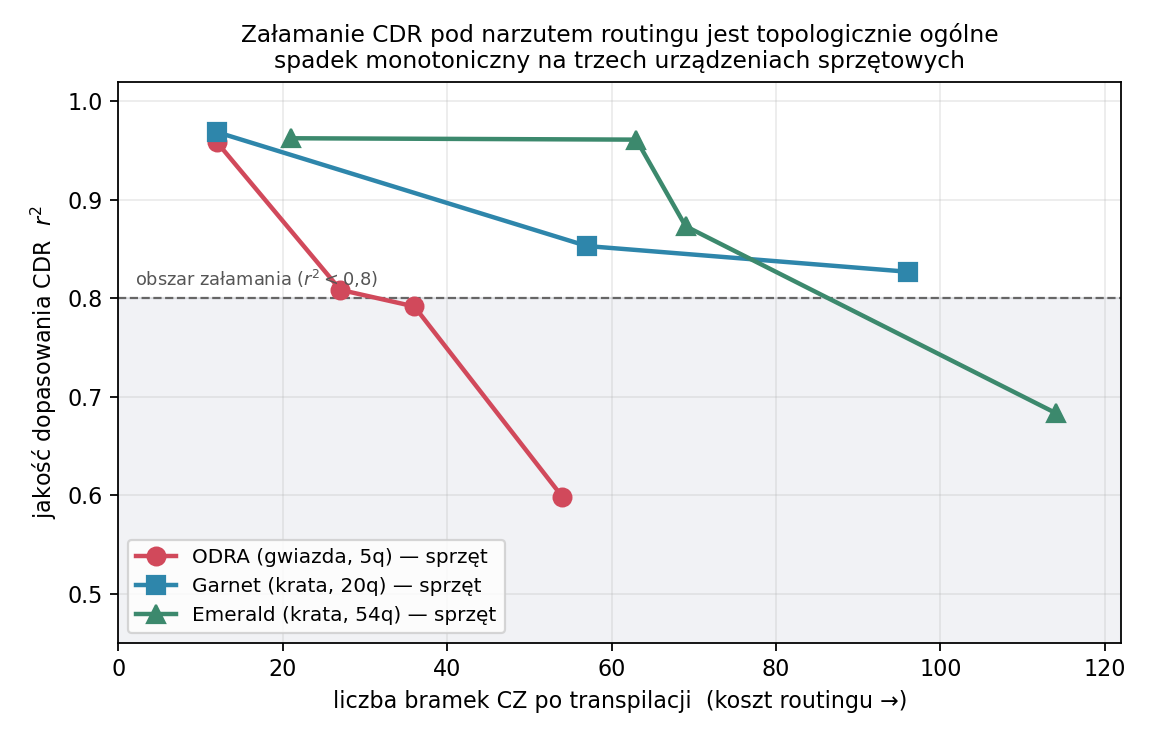
\includegraphics[width=0.75\textwidth]{fig1_cross_topology.png}
  \caption{Jakość dopasowania CDR ($r^2$) w funkcji liczby bramek CZ po transpilacji, dla trzech
  topologii nadprzewodzących. Obszar zacieniony oznacza region załamania ($r^2<0{,}8$), w którym
  liniowe założenie CDR przestaje być spełnione. Wartości dla Garneta uśredniono po trzech oknach
  kalibracyjnych. Wszystkie trzy krzywe pochodzą z~pomiarów na rzeczywistych urządzeniach.}
  \label{fig:xtopo}
\end{figure}

\paragraph{Obserwacja główna.} Na \emph{wszystkich trzech} topologiach $r^2$ spada monotonicznie
z~kosztem routingu. Załamanie
nie jest więc artefaktem jednego urządzenia ani jednej kraty -- jest \textbf{topologicznie ogólne}.
Ponieważ struktura obwodu logicznego, model, obserwabl i metryka są identyczne, jedyną zmienną
odpowiedzialną za tę degradację pozostaje narzut routingu.

Spadek nie jest przy tym gładki w~liczbie bramek. Na Emeraldzie przejście z~21 do 63~CZ, a~więc
potrojenie kosztu routingu, obniża $r^2$ zaledwie o~$0{,}001$; degradacja przyspiesza dopiero
powyżej tego zakresu. Sugeruje to, że koherencja musi najpierw skumulować się do pewnego poziomu,
zanim zacznie mierzalnie naruszać liniowość -- co jest spójne z~kwadratową zależnością od liczby
bramek wyprowadzoną w~Sekcji~\ref{sec:taksonomia}.

\paragraph{Różnice tempa.} Topologie różnią się \emph{szybkością} wchodzenia w region załamania.
Interpolując liniowo między zmierzonymi punktami, gwiazda przekracza próg $r^2<0{,}8$ w~okolicy
\textbf{32~CZ}, Emerald dopiero przy \textbf{86~CZ}, a~Garnet nie schodzi poniżej progu w~całym
zbadanym zakresie (minimum $0{,}827$ przy 96~CZ). Jest to spójne z~geometrią: na gwieździe każda
operacja między kubitami zewnętrznymi musi przejść przez węzeł centralny, co szybko mnoży liczbę
bramek SWAP. \emph{Zastrzeżenie:} próg dla Garneta jest \emph{dolnym ograniczeniem} -- drabina tego
urządzenia kończy się na 96~CZ, więc przecięcie mogło po prostu nie zostać osiągnięte.

\paragraph{Wniosek praktyczny: budżet bramek jest specyficzny dla topologii.} Ta sama liczba bramek
CZ oznacza inny stopień degradacji na gwieździe niż na kracie, więc próg opłacalności trzeba
wyznaczać osobno dla każdego urządzenia -- ale \emph{kształt} zależności jest wspólny, co pozwala
przenosić samą procedurę wyznaczania progu.

% =====================================================================================
\section{Wynik 2: mechanizmem jest błąd koherentny}\label{sec:mechanizm}

Monotoniczny spadek $r^2$ mówi, że wraz z narzutem routingu \emph{coś} narusza założenie liniowości
CDR. Aby wykazać, że tym czymś jest błąd \emph{koherentny}, przeprowadzono eksperyment
symulacyjny, w którym znamy naturę szumu, a protokół pomiarowy jest identyczny jak na sprzęcie
(te same parametry, ta sama kontrola zrównana na liczbie pomiarów, te same okna).

\begin{table}[h]\centering
\caption{Symulacja towarzysząca: zysk twirlingu $\Delta r^2 = r^2(\text{ON}) - r^2(\text{OFF})$ przy
kontroli zrównanej na liczbie pomiarów, w trzech reżimach szumu. Niepewności to odchylenia
standardowe między oknami. Pod szumem niekoherentnym twirling nie przynosi zysku; pod szumem
koherentnym zysk rośnie z~kosztem routingu i skaluje się z~amplitudą koherencji.}
\label{tab:mechanizm}
\begin{tabular}{lcccc}
\toprule
Reżim szumu & 33 CZ & 87 CZ & 90 CZ & trend (na 100 CZ) \\
\midrule
depolaryzacja (kontrola zerowa) & $-0{,}001 \pm 0{,}005$ & $-0{,}003 \pm 0{,}030$ & $-0{,}018 \pm 0{,}049$ & $-0{,}019 \pm 0{,}065$ \\
koherentny, $\theta=0{,}05$ & $+0{,}034 \pm 0{,}007$ & $+0{,}235 \pm 0{,}005$ & $+0{,}140 \pm 0{,}004$ & $+0{,}270 \pm 0{,}015$ \\
koherentny, $\theta=0{,}10$ & $+0{,}157 \pm 0{,}024$ & $+0{,}571 \pm 0{,}022$ & $+0{,}484 \pm 0{,}008$ & $+0{,}659 \pm 0{,}034$ \\
\bottomrule
\end{tabular}
\end{table}

\paragraph{Kontrola zerowa.} Pod szumem czysto depolaryzującym -- niekoherentnym z definicji --
zysk twirlingu jest zgodny z zerem lub nieznacznie ujemny w~całym zakresie, a jego trend względem
kosztu routingu jest płaski ($-0{,}019 \pm 0{,}065$). Nieznaczna ujemność jest zresztą oczekiwana:
obwód otwirlowany zawiera dodatkowe bramki Pauliego, które same wnoszą trochę szumu. Kontrola ta
pełni w~pracy podwójną rolę: dowodzi, że protokół nie wytwarza zysku tam, gdzie go być nie powinno,
i~wyznacza \emph{poziom zerowy} (rzędu $\pm 0{,}03$--$0{,}05$ przy wysokim koszcie routingu), który
wynik sprzętowy musi przekroczyć.

\paragraph{Kontrola pozytywna i zależność dawka--odpowiedź.} Po wstrzyknięciu koherentnego obrotu
nadmiarowego na każdej bramce CZ obraz zmienia się jakościowo: zysk twirlingu jest dodatni, istotny
i~\emph{rośnie z~kosztem routingu} (trend $+0{,}270 \pm 0{,}015$ przy $\theta=0{,}05$). Podwojenie
amplitudy koherencji zwiększa zysk 2{,}4--4{,}6-krotnie -- zależność dawka--odpowiedź, której szum
niekoherentny nie odtwarza w~żadnym stopniu. Reżim $\theta=0{,}05$ odpowiada przy tym warunkom
sprzętowym: $r^2$ ramienia nietwirlowanego spada w nim z 0{,}94 do 0{,}75 wzdłuż drabiny, co
odpowiada obserwowanemu na Garnecie spadkowi z~0{,}98 do 0{,}79.

\paragraph{Pomiar koherencji na poziomie bramki.} Niezależnie wykonano \emph{unitarity randomized
benchmarking}~\cite{wallman2015} na parze kubitów Garneta, uzyskując unitarność $u=0{,}843$ przy
zaniku standardowego RB $p=0{,}908$ (a więc $p^2=0{,}824$). Nadwyżka $u-p^2 = +0{,}019$ wskazuje na
niewielki udział błędu koherentnego \emph{pojedynczej bramki}, przy czym dryf tej wielkości między
oknami ($\approx 0{,}09$) znacznie przewyższa sam sygnał. Wniosek jest zatem ograniczający, ale
istotny: koherencja izolowanej bramki CZ jest mała, więc obserwowany zysk twirlingu musi pochodzić
z~poziomu \emph{obwodu} -- z~kumulacji na łańcuchach SWAP, okresach bezczynności i przesłuchach --
a nie z pojedynczej operacji. Ilościowe domknięcie tej ścieżki (przewidziany $=$ zmierzony zysk)
wymagałoby \emph{cycle benchmarkingu} na poziomie warstwy i pozostaje zadaniem otwartym.

\begin{figure}[h]\centering
  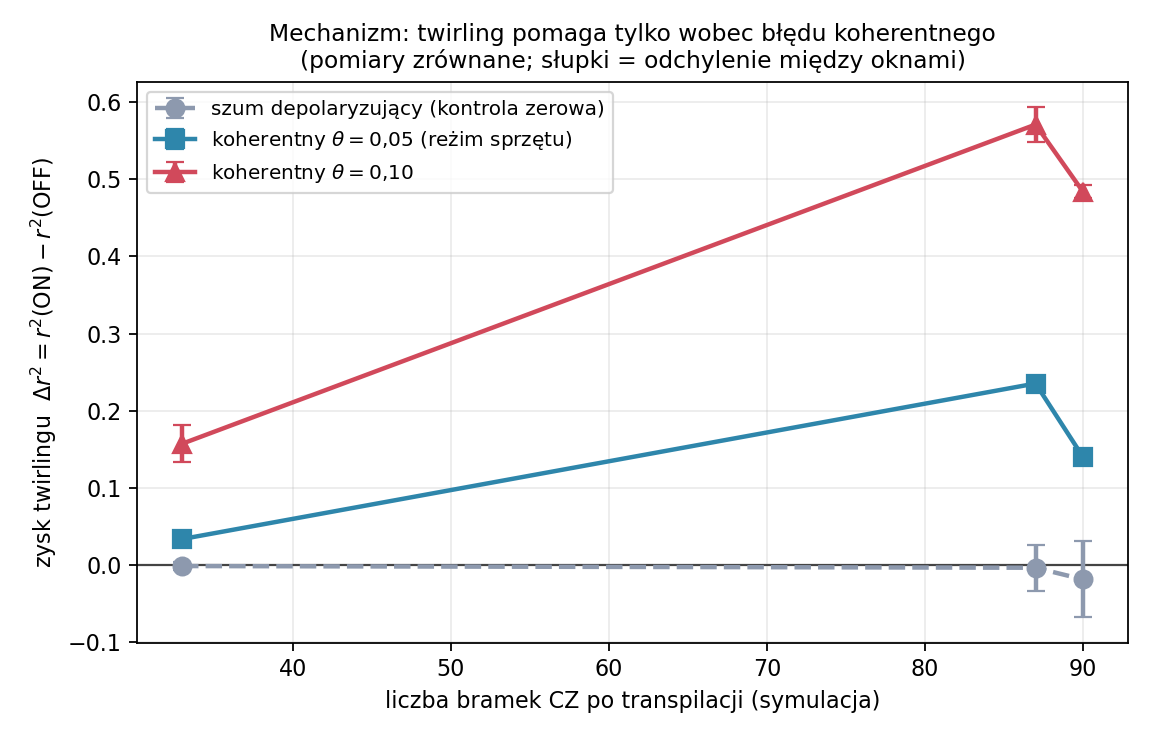
\includegraphics[width=0.72\textwidth]{fig2_companion_sim.png}
  \caption{Symulacja towarzysząca: zysk twirlingu $\Delta r^2$ w funkcji kosztu routingu dla trzech
  reżimów szumu, przy kontroli zrównanej na liczbie pomiarów. Pod szumem niekoherentnym efekt jest
  zgodny z~zerem i~pozbawiony trendu; pod szumem koherentnym rośnie z~kosztem routingu i~skaluje się
  z~amplitudą koherencji (zależność dawka--odpowiedź).}
  \label{fig:companion}
\end{figure}

\paragraph{Wniosek praktyczny: $r^2$ jest tanią sondą charakteru szumu.} Skoro spadek $r^2$ jest
sygnaturą koherencji, a~nie ogólnego ,,pogorszenia'', to samo dopasowanie CDR -- które i~tak trzeba
wykonać, żeby metody użyć -- mówi za darmo, czy w~obwodzie warto uruchamiać twirling.

Wartość tej obserwacji bierze się z~porównania z~alternatywami. Żeby dowiedzieć się, jaka część
błędu urządzenia jest koherentna, trzeba normalnie wykonać \emph{osobny eksperyment}: unitarity
randomized benchmarking albo cycle benchmarking. Oba wymagają własnych obwodów, własnego czasu
maszynowego i~własnej analizy, a~ich wynik dotyczy \emph{bramki} lub \emph{warstwy} -- nie tego
konkretnego obwodu, który ma zostać uruchomiony. Widać to na własnym pomiarze: unitarity
RB dało nadwyżkę koherentną $+0{,}019$ przy dryfie między oknami rzędu $0{,}09$, czyli sygnał
\emph{utonął} w~dryfie i~nie pozwolił przewidzieć niczego o~pojedynczym przebiegu.

Współczynnik $r^2$ nie ma żadnej z~tych wad. Jest liczony na \emph{tym samym} obwodzie, w~\emph{tym
samym} oknie kalibracyjnym i~z~\emph{tych samych} pomiarów, które i~tak trzeba wykonać -- koszt
dodatkowy wynosi zero. Mierzy przy tym dokładnie tę wielkość, która decyduje o~opłacalności
interwencji, a~nie jej pośrednik: liczba bramek CZ mówi, ile koherencji \emph{mogło} narosnąć,
podczas gdy $r^2$ mówi, ile jej \emph{jest} -- w~tym przebiegu, przy tym stanie urządzenia. To
dlatego zysk z~twirlingu koreluje z~$r^2$, a~z~liczbą bramek już nie
(Sekcja~\ref{sec:twirl-wynik}).

% =====================================================================================
\section{Wynik 3: twirling przywraca skuteczność CDR na sprzęcie}\label{sec:twirl-wynik}

Jeżeli mechanizmem załamania jest błąd koherentny, to konwersja tego błędu na stochastyczny powinna
przywrócić liniowość CDR -- i to tym silniej, im większy narzut routingu. Hipotezę tę zweryfikowano
na żywym urządzeniu Garnet.

\begin{table}[h]\centering
\caption{Garnet: sparowany zysk twirlingu przy kontroli zrównanej na liczbie pomiarów, z~trzech
okien kalibracyjnych. Niepewności to odchylenia standardowe między oknami.}
\label{tab:twirl}
\begin{tabular}{rcccl}
\toprule
CZ & $\Delta r^2$ & $\Delta \varepsilon$ & wartości w~oknach & werdykt \\
\midrule
12 & $+0{,}016 \pm 0{,}019$ & $-0{,}024 \pm 0{,}022$ & $-0{,}001$; $+0{,}012$; $+0{,}036$ & w~poziomie zerowym \\
57 & $+0{,}069 \pm 0{,}023$ & $-0{,}016 \pm 0{,}019$ & $+0{,}090$; $+0{,}044$; $+0{,}074$ & \textbf{istotny} \\
96 & $+0{,}073 \pm 0{,}108$ & $-0{,}027 \pm 0{,}028$ & $+0{,}039$; $+0{,}194$; $-0{,}013$ & nierozstrzygnięty \\
\bottomrule
\end{tabular}
\end{table}

\paragraph{Wynik zgodny z~przewidywaniem mechanizmu -- i jego granice.} Przy najniższym koszcie
routingu (12~CZ) zysk mieści się w~poziomie zerowym ($+0{,}016 \pm 0{,}019$), co jest oczekiwane:
obwód jest zbyt płytki, by koherencja zdążyła się skumulować. Przy 57~CZ zysk jest
\textbf{istotny} ($+0{,}069 \pm 0{,}023$) i~\emph{dodatni we wszystkich trzech oknach}
($+0{,}090$; $+0{,}044$; $+0{,}074$), przekraczając poziom zerowy wyznaczony symulacyjnie. Punkt
96~CZ pozostaje jednak \textbf{nierozstrzygnięty}: rozrzut między oknami ($+0{,}039$; $+0{,}194$;
$-0{,}013$) jest większy niż sam efekt. W~konsekwencji \emph{trend względem liczby bramek CZ nie jest
istotny statystycznie} (Spearman $\rho=+0{,}32$, $p=0{,}41$; $n=9$). Twirling pomaga zatem istotnie w~reżimie pośredniego kosztu routingu, natomiast przy koszcie
najwyższym dryf kalibracyjny dominuje nad efektem.

\begin{figure}[h]\centering
  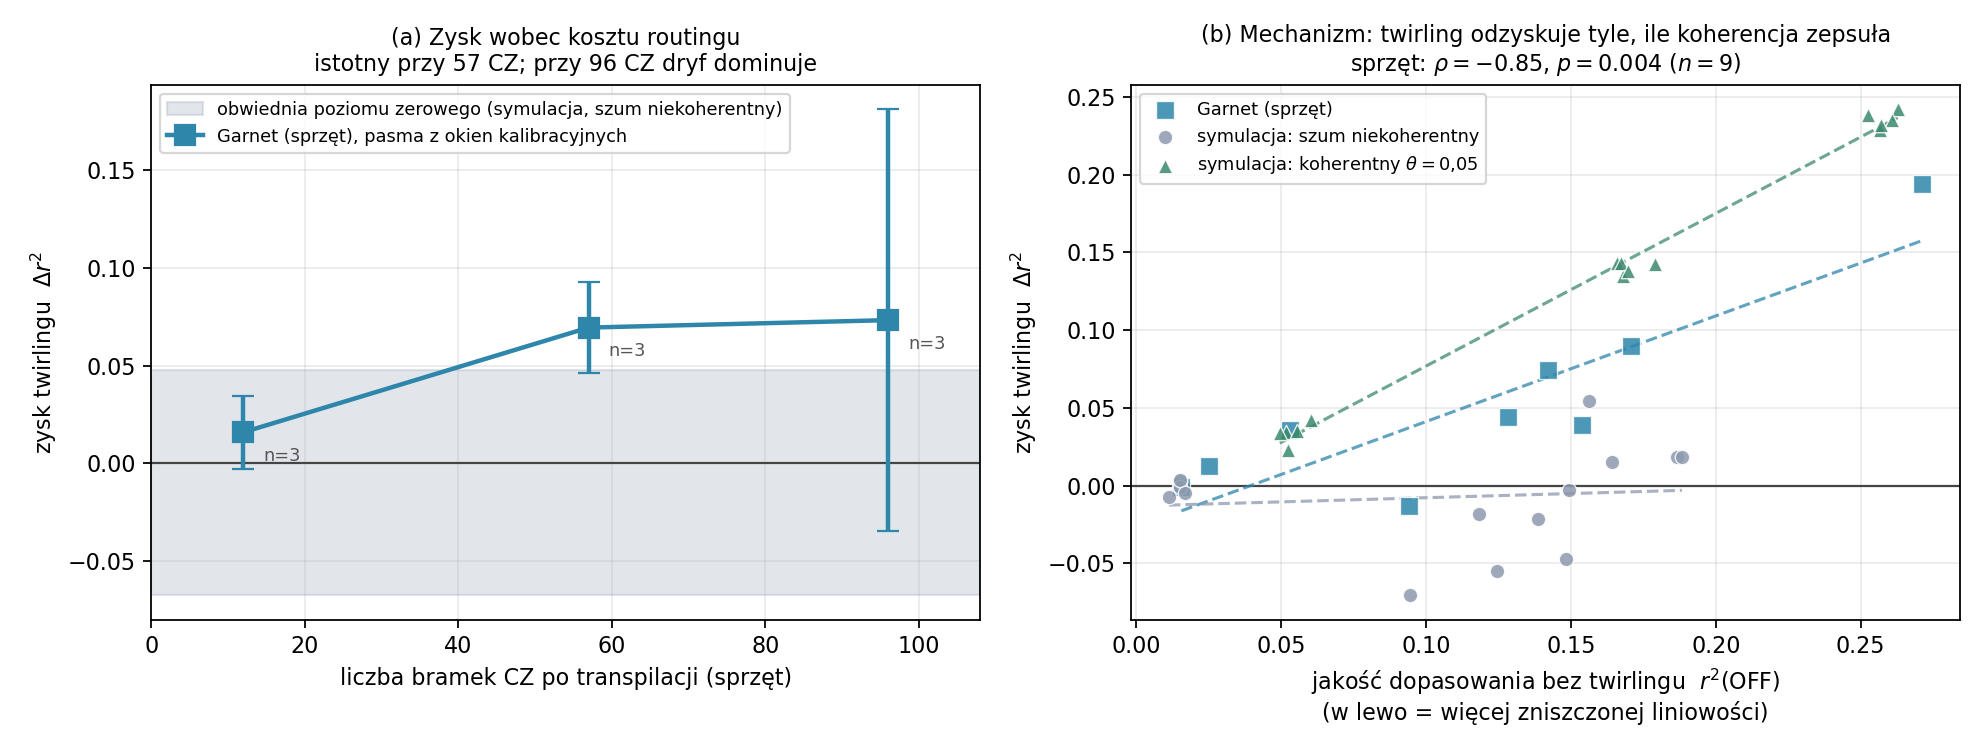
\includegraphics[width=\textwidth]{fig3_twirl_hardware.png}
  \caption{(a) Zysk twirlingu wobec kosztu routingu z~pasmami dryfu; istotny przy 57~CZ, przy 96~CZ
  zdominowany przez dryf. (b) Ten sam zbiór punktów przedstawiony wobec jakości dopasowania bez
  twirlingu: zysk jest \emph{przewidywalny} z~$r^2(\mathrm{OFF})$ i~rośnie w~lewo, czyli tam, gdzie
  koherencja bardziej zepsuła liniowość; punkty sprzętowe układają się między symulacją
  niekoherentną a~koherentną.}
  \label{fig:twirl}
\end{figure}

\paragraph{Właściwym predyktorem nie jest liczba bramek, lecz zniszczenie liniowości.} Duży rozrzut
przy 96~CZ ma konkretne wyjaśnienie: w~trzech oknach urządzenie znajdowało się w~wyraźnie różnym
stanie, a~$r^2$ ramienia nietwirlowanego wynosiło odpowiednio 0{,}846, 0{,}729 i~0{,}906. W~oknie
najgorszym zysk był największy ($+0{,}194$), w~najlepszym -- zerowy ($-0{,}013$). Sugeruje to, że
wielkością sterującą jest nie sam koszt routingu, lecz \emph{ilość koherencji faktycznie obecnej
w~danym oknie}. Dane są z~tą hipotezą zgodne: dla wszystkich dziewięciu pomiarów sprzętowych
(3 punkty $\times$ 3 okna) zysk twirlingu koreluje z~jakością dopasowania bez twirlingu na poziomie
$\rho = -0{,}85$ ($p = 0{,}004$), podczas gdy korelacja z~liczbą bramek CZ jest nieistotna
($\rho = +0{,}32$, $p = 0{,}41$). \textbf{Twirling odzyskuje dokładnie tyle, ile
koherencja wcześniej zepsuła}, a~liczba bramek CZ jest jedynie zaszumionym pośrednikiem tej
wielkości -- zaszumionym, ponieważ stan urządzenia dryfuje między oknami.

\paragraph{Kontrola artefaktu regresji do średniej.} Korelowanie różnicy $\Delta = \mathrm{ON}-\mathrm{OFF}$
z~samym $\mathrm{OFF}$ jest podatne na sprzężenie matematyczne: szum pomiarowy w~$r^2(\mathrm{OFF})$
wchodzi do obu wielkości z~przeciwnymi znakami, wytwarzając ujemną korelację nawet przy braku
efektu. Wielkość tego artefaktu zmierzono bezpośrednio na danych kontrolnych: w~symulacji z~szumem
niekoherentnym ($n=15$) korelacja wynosi zaledwie $\rho = -0{,}39$ i~\emph{nie jest istotna}
($p = 0{,}16$). Wynik sprzętowy ($-0{,}85$) znacznie ten poziom przekracza i~odpowiada reżimom
z~wstrzykniętą koherencją ($-0{,}91$ dla $\theta=0{,}05$; $-0{,}82$ dla $\theta=0{,}10$), co widać
także na Rysunku~\ref{fig:twirl}(b) jako nachylenie prostych dopasowania. Zależność nie jest zatem
artefaktem statystycznym.

\emph{Zakres wniosku.} Korelacja opiera się na dziewięciu pomiarach (3 punkty drabiny $\times$
3 okna kalibracyjne), co jest liczebnością małą -- przy takim $n$ sam współczynnik Spearmana ma
istotną wariancję i~pojedynczy odstający punkt drabiny mógłby go zauważalnie przesunąć. Zależność tę traktuje
się zatem jako wynik wstępny, wsparty jednak spójnym obrazem: wartość sprzętowa $-0{,}85$ leży
wyraźnie powyżej poziomu kontroli zerowej ($-0{,}39$, nieistotne) i~w~przedziale wyznaczonym przez
oba reżimy wstrzykniętej koherencji ($-0{,}91$ i~$-0{,}82$). Rozszerzenie drabiny o~punkty
pośrednie w~kolejnych oknach kalibracyjnych jest naturalnym sposobem domknięcia tej kwestii.

\paragraph{Kalibracja skali koherencji.} Średni zysk twirlingu układa się monotonicznie wzdłuż
reżimów: $-0{,}008$ (szum niekoherentny), $+0{,}053$ (Garnet), $+0{,}137$ ($\theta=0{,}05$),
$+0{,}404$ ($\theta=0{,}10$). Umiejscawia to Garnet \emph{powyżej} poziomu niekoherentnego, lecz
\emph{poniżej} najsłabszej wstrzykniętej koherencji, co odpowiada efektywnej amplitudzie rzędu
$\theta \approx 0{,}02$--$0{,}03$~rad na bramkę dwukubitową. Jest to zgodne z~niezależnym pomiarem
unitarity RB (Sekcja~\ref{sec:mechanizm}), według którego koherencja pojedynczej bramki jest
niewielka, co potwierdza, że obserwowany efekt gromadzi się na poziomie obwodu.

\subsection*{Reguła decyzyjna: zmierz \texorpdfstring{$r^2$}{r2}, nie licz bramek}

Wyniki tej sekcji składają się w~jedno stwierdzenie, które uważamy za najbardziej użytkowy wniosek
całej pracy:

\begin{center}
\fbox{\parbox{0.92\textwidth}{\vspace{2pt}
\textbf{Twirling odzyskuje dokładnie tyle, ile koherencja wcześniej zepsuła.} Wielkością sterującą
nie jest koszt routingu, lecz stopień naruszenia liniowości -- mierzalny \emph{przed} podjęciem
decyzji, za darmo, jako $r^2$ zwykłego dopasowania CDR.
\vspace{4pt}

\emph{Reguła:} dopasuj CDR bez twirlingu i~odczytaj $r^2$. Przy $r^2 \gtrsim 0{,}95$ twirling nie
ma czego naprawiać -- zysk mieści się w~poziomie zerowym, a~$M$-krotny narzut pomiarowy zostaje.
Przy $r^2 \lesssim 0{,}90$ narosła koherencja i~twirling ją usuwa: w~zebranych pomiarach odzyskał
$\Delta r^2 = +0{,}069 \pm 0{,}023$ przy $r^2(\mathrm{OFF}) = 0{,}853$.
\vspace{2pt}}}
\end{center}

Wartość tej reguły polega na tym, że \emph{odwraca kolejność} zwykłego rozumowania. Naturalny
odruch -- ,,obwód ma dużo bramek, więc pewnie warto twirlować'' -- w~zebranych danych zawodzi:
korelacja zysku z~liczbą bramek CZ nie osiąga istotności ($\rho=+0{,}32$, $p=0{,}41$), ponieważ
liczba bramek mówi o~\emph{potencjale} kumulacji koherencji, a~nie o~tym, ile jej faktycznie narosło
w~danym oknie kalibracyjnym. Stan urządzenia dryfuje, więc ten sam obwód bywa raz mocno, a~raz słabo
dotknięty, co widać wprost w~danych: przy 96~CZ ten sam punkt drabiny dał w~trzech oknach zyski
$+0{,}039$, $+0{,}194$ i~$-0{,}013$. Liczba bramek była za każdym razem identyczna; różniła się
\emph{koherencja}, a~$r^2$ ją wychwyciło.

Praktyczna konsekwencja jest taka, że użytkownik nie musi ani znać modelu szumu swojego urządzenia,
ani wykonywać osobnego eksperymentu benchmarkingowego, żeby zdecydować o~zastosowaniu twirlingu.
Wystarczy, że i~tak stosuje CDR -- wtedy diagnostyka jest gotowa, zanim wyda pierwszy dodatkowy
pomiar.

% =====================================================================================
\section{Wynik 4: progi rozdzielone po urządzeniach}\label{sec:progi}

Poprzednie sekcje opisują mechanizm i~jego neutralizację; ta umieszcza je w~kontekście
praktycznym: \emph{która metoda opłaca się przy jakim budżecie bramek}. Tabela~\ref{tab:progi}
zestawia wszystkie trzy podejścia na wspólnej osi kosztu.

\begin{table}[h]\centering
\caption{Błąd $\varepsilon$ bez mitygacji, po CDR i po ZNE wzdłuż drabin routingu trzech urządzeń.
Pogrubiono metodę najlepszą w~danym punkcie.}
\label{tab:progi}
\begin{tabular}{lrcccl}
\toprule
Urządzenie & CZ & bez mitygacji & CDR & ZNE & najlepsza \\
\midrule
ODRA    &  12 & 0{,}075 & 0{,}027 & \textbf{0{,}023} & ZNE \\
        &  27 & 0{,}150 & \textbf{0{,}071} & 0{,}090 & CDR \\
        &  36 & 0{,}186 & \textbf{0{,}105} & 0{,}142 & CDR \\
        &  54 & 0{,}278 & 0{,}220 & 0{,}219 & \emph{remis} \\
\midrule
Garnet  &  12 & 0{,}073 & 0{,}049 & \textbf{0{,}031} & ZNE \\
        &  57 & 0{,}127 & \textbf{0{,}058} & 0{,}081 & CDR \\
        &  96 & 0{,}111 & \textbf{0{,}058} & 0{,}103 & CDR \\
\midrule
Emerald &  21 & 0{,}037 & \textbf{0{,}024} & 0{,}168 & CDR (ZNE szkodzi) \\
        &  63 & 0{,}101 & \textbf{0{,}070} & 0{,}077 & CDR \\
        &  69 & 0{,}079 & 0{,}059 & \textbf{0{,}049} & ZNE \\
        & 114 & \textbf{0{,}101} & 0{,}279 & 0{,}139 & \emph{kolaps} \\
\bottomrule
\multicolumn{6}{l}{\footnotesize Wszystkie wartości pochodzą z~pomiarów sprzętowych; dla każdego
urządzenia}\\
\multicolumn{6}{l}{\footnotesize wszystkie trzy metody zmierzono w~jednej kampanii i~jednym oknie
kalibracyjnym.}
\end{tabular}
\end{table}

\begin{figure}[h]\centering
  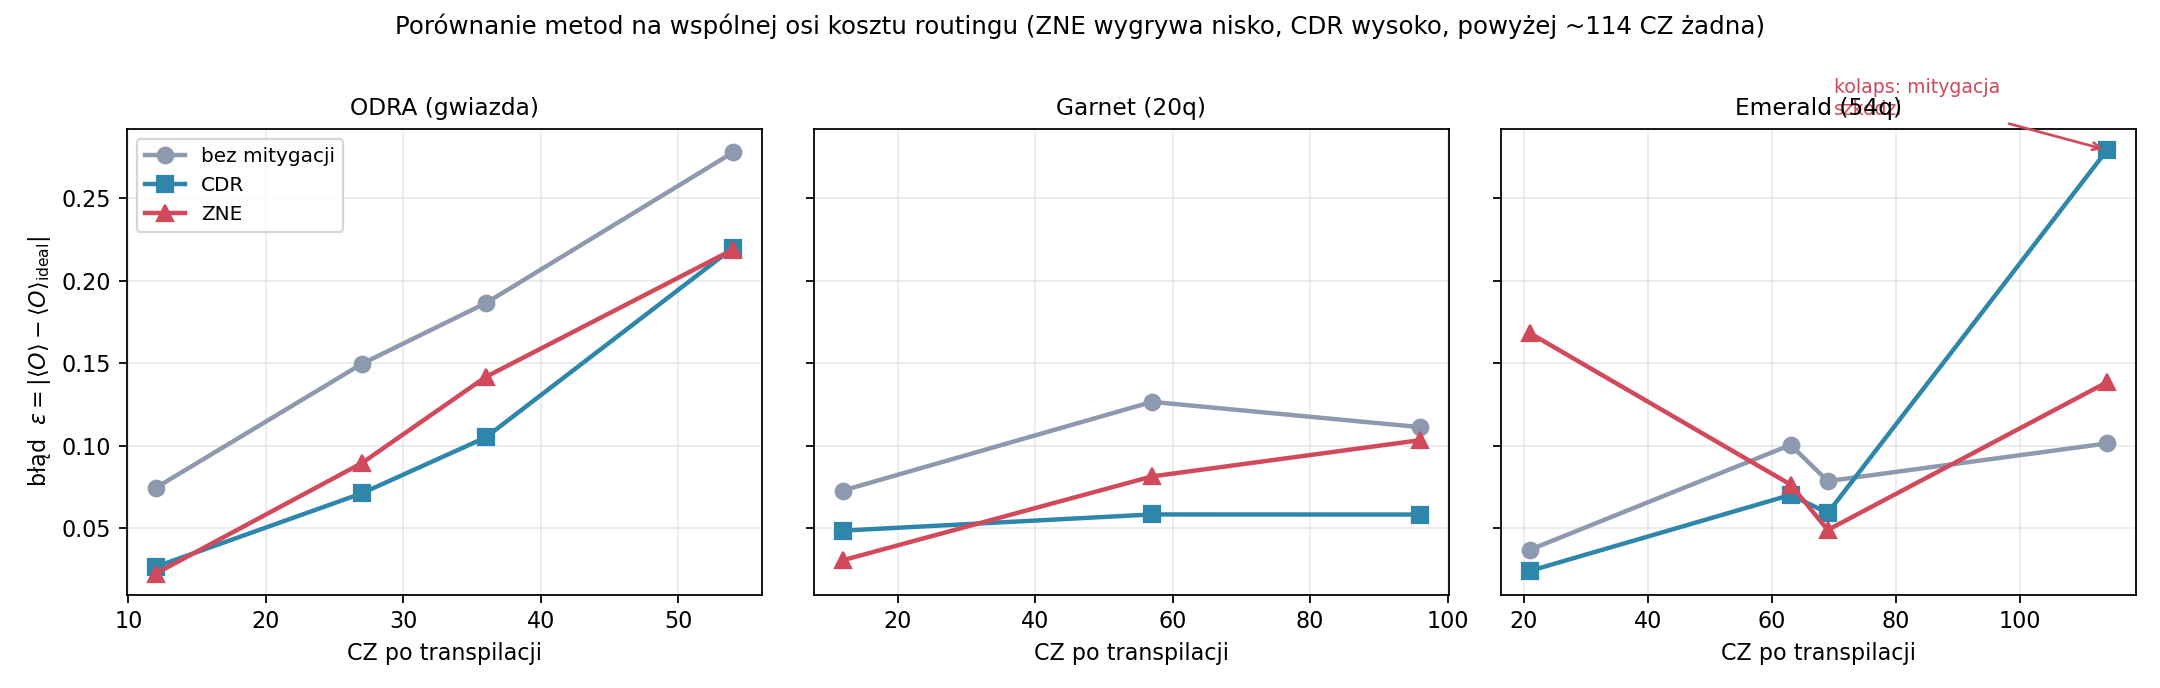
\includegraphics[width=\textwidth]{fig4_method_comparison.png}
  \caption{Błąd $\varepsilon$ bez mitygacji, po CDR i po ZNE wzdłuż drabin routingu trzech urządzeń.
  ZNE wygrywa przy niskim koszcie routingu, CDR przy wyższym; przy 114~CZ (Emerald) żadna metoda nie
  przewyższa wyniku niemitygowanego.}
  \label{fig:metody}
\end{figure}

\paragraph{Punkt równowagi ZNE\,$\leftrightarrow$\,CDR.} Przy niskim koszcie routingu wygrywa ZNE
(12~CZ na ODRZE i~na Garnecie), przy wyższym -- CDR. Niezależna analiza kosztowa na Garnecie
umiejscawia punkt równowagi w okolicy \textbf{39~CZ}. Wybór metody nie jest przy tym neutralny
kosztowo: przy parametrach kampanii obu metod (ZNE: 4096 pomiarów $\times$ 3 skale; CDR: 2048
pomiarów $\times$ 41 obwodów, czyli 40 treningowych i~docelowy) ZNE zużywa 12\,288 efektywnych
pomiarów wobec 83\,968 dla CDR, a~więc blisko siedmiokrotnie mniej. Poniżej punktu równowagi ZNE jest zatem zarówno \emph{lepsze},
jak i~\emph{tańsze}; powyżej trzeba dopłacić za CDR, aby cokolwiek zyskać.

\paragraph{ZNE bywa szkodliwe -- granica help--harm.} Na Emeraldzie przy 21~CZ ekstrapolacja
Richardsona daje błąd 0{,}168 wobec 0{,}037 bez jakiejkolwiek mitygacji -- pogorszenie ponad
czterokrotne. Nie jest to anomalia, a~empiryczna granica: przy ustalonym budżecie pomiarów wzmocniona
wariancja próbkowania dominuje nad redukowanym obciążeniem~\cite{alfaro2026}. Punkt
ten jest w~tym badaniu \emph{najmniej} zaszumiony (błąd bez mitygacji 0{,}037) i~zmierzony przy
zaledwie 2048 pomiarach, a~więc leży dokładnie po ,,szkodliwej'' stronie granicy. Obserwacja ta
zamyka oś opłacalności z~drugiej strony: ZNE ma nie tylko górny próg (kolaps sygnału, poniżej), lecz
także \emph{dolny} -- przy zbyt małym szumie i skończonej statystyce lepiej nie mitygować wcale.

\paragraph{Granica opłacalności -- prognoza pre-rejestrowana.} Warunek wyprowadzony
w~Sekcji~\ref{sec:metody-mitygacji} można zapisać jako granicę na obciążenie przy ustalonym budżecie
pomiarów $S$,
\begin{equation}
  B^{*} \;=\; \sqrt{\frac{\kappa\,V}{S}}, \qquad
  \kappa = \Bigl(\textstyle\sum_i c_i^2\Bigr)\,|\Lambda| - 1 = 14{,}66 ,
  \label{eq:granica}
\end{equation}
lub równoważnie jako budżet krytyczny $S^{*} = \kappa V / B^2$ dla danego punktu drabiny. Skonfrontowanie
tego przewidywania z~danymi zebranymi w~kampanii głównej (Tabela~\ref{tab:granica}) daje zgodność
w~sześciu na siedem punktów, przy czym jedyna rozbieżność -- Emerald przy 114~CZ -- jest punktem
niezależnie zdiagnozowanym jako kolaps sygnału ($R=0{,}15$), a~więc podlegającym \emph{drugiemu}
mechanizmowi. Oba mechanizmy razem wyjaśniają wszystkie siedem obserwacji. Szczególnie wymowny jest
punkt Emerald 21~CZ, w~którym zmierzone obciążenie $0{,}0370$ leży praktycznie na przewidzianej
granicy $0{,}0378$, i~w~którym ZNE faktycznie zaszkodziło.

\begin{table}[h]\centering
\caption{Przewidywanie granicy~\eqref{eq:granica} wobec danych. Wartość $V\approx0{,}2$ oszacowano
analitycznie dla obserwabla średniego~$Z$ na pięciu kubitach; nie dopasowywano żadnego parametru
do~danych.}
\label{tab:granica}
\begin{tabular}{lrrccll}
\toprule
Urządzenie & CZ & $S$ & $B$ & $B^{*}$ & przewidywanie & obserwacja \\
\midrule
Emerald & 21 & 2048 & 0{,}0370 & 0{,}0378 & zaszkodzi & zaszkodziło \\
Emerald & 63 & 2048 & 0{,}1005 & 0{,}0378 & pomoże & pomogło \\
Emerald & 69 & 2048 & 0{,}0786 & 0{,}0378 & pomoże & pomogło \\
Emerald & 114 & 2048 & 0{,}1014 & 0{,}0378 & pomoże & \emph{zaszkodziło} (kolaps) \\
Garnet & 12 & 1024 & 0{,}0729 & 0{,}0535 & pomoże & pomogło \\
Garnet & 57 & 1024 & 0{,}1266 & 0{,}0535 & pomoże & pomogło \\
Garnet & 96 & 1024 & 0{,}1113 & 0{,}0535 & pomoże & pomogło \\
\bottomrule
\end{tabular}
\end{table}

Powyższa zgodność opiera się jednak na pojedynczym przejściu granicy. Ostrzejszym testem jest
pomiar \emph{całej krzywej przejścia}: dla ustalonego punktu drabiny zwiększamy budżet pomiarów
i~sprawdzamy, przy jakiej jego wartości ZNE przestaje szkodzić, a~zaczyna pomagać. Zapisujemy zatem
prognozę \emph{przed} wykonaniem pomiaru, w~postaci, która nie zawiera żadnego parametru
dopasowywanego do danych:
\begin{quote}
\textbf{Prognoza pre-rejestrowana.} Ponieważ ekstrapolacja z~trzech węzłów usuwa jedynie dwa
pierwsze rzędy rozwinięcia~\eqref{eq:zne-exp}, ramię ZNE zachowuje obciążenie resztkowe
$B_{\text{zne}}$, a~różnica błędów średniokwadratowych przyjmuje postać liniową w~budżecie:
\begin{equation}
  \bigl(\text{MSE}_{\text{ZNE}} - \text{MSE}_{\text{raw}}\bigr)\cdot S
  \;=\; \underbrace{\kappa V}_{\text{wyraz wolny}}
  \;-\; \underbrace{\bigl(B^2 - B_{\text{zne}}^2\bigr)}_{\text{nachylenie}}\, S .
  \label{eq:kappa-fit}
\end{equation}
Przewidujemy, że dopasowanie prostej do zmierzonych punktów da wyraz wolny równy $\kappa V$ ze
\emph{stałą} $\kappa = 14{,}66$, wynikającą wyłącznie z~wyboru węzłów $\{1,3,5\}$, przy czym $V$
wyznaczymy niezależnie z~rozkładu zliczeń w~tym samym przebiegu. Falsyfikowalna jest zatem sama
stała $\kappa$, a~nie konkretna wartość budżetu krytycznego. Nachylenie dostarcza dodatkowo pomiaru
tego, \emph{jaką część} obciążenia ekstrapolacja faktycznie usuwa, oraz kontroli krzyżowej wobec
obciążenia zmierzonego bezpośrednio.
\end{quote}
\paragraph{Wynik testu.} Kampanię wykonano na Garnecie w~dwóch punktach drabiny o~różnym
obciążeniu, przy budżetach 96--2048 pomiarów, 12 powtórzeniach i~6 punktach ewaluacyjnych
(Tabela~\ref{tab:kappa}). Prognoza została potwierdzona.

\begin{table}[h]\centering
\caption{Wynik testu pre-rejestrowanej prognozy. Wartość $\kappa$ wyznaczono z~wyrazu wolnego
dopasowania~\eqref{eq:kappa-fit}, przy $V$ zmierzonym niezależnie z~rozkładu zliczeń. Żaden parametr
nie był dopasowywany do danych.}
\label{tab:kappa}
\begin{tabular}{lccccc}
\toprule
Punkt & CZ & $B$ & $V$ & $\kappa$ zmierzone & odchylenie \\
\midrule
\texttt{optimal:star} & 12 & 0{,}056 & 0{,}193 & $14{,}42 \pm 0{,}95$ & $0{,}25\sigma$ \\
\texttt{adverse:star} & 48 & 0{,}100 & 0{,}202 & $13{,}29 \pm 1{,}73$ & $0{,}79\sigma$ \\
\midrule
\multicolumn{4}{l}{\textbf{średnia ważona}} & $\mathbf{14{,}16 \pm 0{,}83}$ & $\mathbf{0{,}60\sigma}$ \\
\bottomrule
\end{tabular}
\end{table}

Wynik jest zgodny z~przewidywaniem $\kappa = 14{,}66$ na poziomie $0{,}60\sigma$. Potwierdzenia
dostarczają ponadto dwie niezależne kontrole. Po pierwsze, zmierzona wariancja obserwabla na pomiar
($V = 0{,}190$--$0{,}206$) pokrywa się z~wartością oszacowaną analitycznie ($0{,}200$). Po drugie --
i~jest to \emph{osobna} falsyfikacja -- teoria przewiduje skalowanie budżetu krytycznego
$S^{*} \propto B^{-2}$. Dla obu punktów stosunek kwadratów obciążeń wynosi $3{,}24$, a~zmierzony
stosunek budżetów krytycznych ($847$ wobec $291$ pomiarów) -- $2{,}91$, czyli zgodność w~granicach
10\%. Przejścia zaobserwowano bezpośrednio: dla \texttt{optimal:star} w~przedziale $(1024, 2048]$,
dla \texttt{adverse:star} w~$(256, 384]$ -- większe obciążenie oznacza wcześniejsze przejście,
zgodnie z~przewidywaniem.

\paragraph{Konsekwencja praktyczna: liczba węzłów przesuwa granicę.} Ponieważ $\kappa$ zależy
wyłącznie od wyboru węzłów, dobór tego zbioru jest \emph{decyzją projektową}, która wprost przesuwa
dolną granicę opłacalności. Dla składania globalnego (dającego wyłącznie skale nieparzyste)
uzyskuje się $\kappa = 4{,}00$ dla $\{1,3\}$, $14{,}66$ dla $\{1,3,5\}$ oraz $44{,}56$ dla
$\{1,3,5,7\}$. Redukcja liczby węzłów z~trzech do dwóch obniża zatem próg budżetowy
$S^{*}=\kappa V/B^2$ blisko czterokrotnie -- kosztem mniejszej redukcji obciążenia, ponieważ
ekstrapolacja usuwa wtedy tylko pierwszy rząd rozwinięcia. W~reżimie płytkich obwodów
i~oszczędnych budżetów pomiarów jest to kompromis wart rozważenia i~stanowi bezpośrednią
rekomendację praktyczną.

\paragraph{Test na drugim zbiorze węzłów.} Dopasowanie jednej stałej do jednego pomiaru zawsze można
uznać za zbieg okoliczności. Powtórzyliśmy więc całą kampanię z~węzłami $\{1,3\}$, dla których
teoria przewiduje $\kappa = 4{,}00$ dokładnie (współczynniki Richardsona $\tfrac{3}{2},
-\tfrac{1}{2}$, zatem $\sum_i c_i^2 = \tfrac{5}{2}$ oraz $\kappa = 2\cdot\tfrac{5}{2}-1$).
Protokół, urządzenie i~analiza pozostały bez zmian; zmienił się wyłącznie zbiór węzłów. Wyniki
zebrano w~Tabeli~\ref{tab:kappa2}.

\begin{table}[h]\centering
\caption{Test ogólności prawa $\kappa$: ta sama procedura, dwa różne zbiory węzłów o~przewidywanych
wartościach różniących się $3{,}66$-krotnie. Wartości zmierzone pochodzą z~wyrazu wolnego
dopasowania~\eqref{eq:kappa-fit}; ponownie żaden parametr nie był dopasowywany do danych.}
\label{tab:kappa2}
\begin{tabular}{lccc}
\toprule
Zbiór węzłów $\Lambda$ & $\kappa$ przewidziane & $\kappa$ zmierzone & odchylenie \\
\midrule
$\{1,3,5\}$ & $14{,}656$ & $14{,}16 \pm 0{,}83$ & $0{,}60\sigma$ \\
$\{1,3\}$   & $4{,}000$  & $3{,}39 \pm 0{,}40$  & $1{,}52\sigma$ \\
\midrule
\multicolumn{2}{l}{\textbf{wspólne dopasowanie} $\kappa_{\text{zmierz}} = s\,\kappa_{\text{przewid}}$}
 & $s = 0{,}937 \pm 0{,}049$ & $1{,}27\sigma$ \\
\bottomrule
\end{tabular}
\end{table}

Oba zbiory węzłów dają wartości zgodne z~przewidywaniami, przy czym zgodny jest sam \emph{stosunek}: teoria przewiduje skok $14{,}656/4{,}000 = 3{,}66$, pomiar daje
$4{,}18 \pm 0{,}55$. Wspólne dopasowanie prostej przez zero do czterech niezależnych punktów
pomiarowych (dwa zbiory węzłów $\times$ dwa punkty drabiny) daje nachylenie $0{,}937 \pm 0{,}049$,
odległe od jedności o~$1{,}27\sigma$, przy $\chi^2/\mathrm{dof} = 0{,}79$. Punkty drabiny użyte w~obu kampaniach różniły się narzutem routingu (12--48 bramek CZ), a~mimo to
dały spójne oszacowania tej samej stałej -- co jest oczekiwane, ponieważ w~modelu cała zależność
od obwodu jest zawarta w~$B$ i~$V$, a~$\kappa$ jest wielkością czysto kombinatoryczną, wynikającą
z~konstrukcji estymatora. Systematyczne, choć nieistotne statystycznie, niedoszacowanie
($s < 1$) jest zgodne z~kierunkiem oczekiwanym przy resztkowym obciążeniu samej ekstrapolacji
(człon $B_{\text{ZNE}}^2$ w~równaniu~\eqref{eq:kappa-fit}), które obniża zmierzony wyraz wolny.

Obserwacja ta ma znaczenie wykraczające poza samą charakterystykę ZNE. Rozwój sprzętu i~algorytmów
zmierza w~stronę obwodów \emph{płytkich} wykonywanych przy \emph{oszczędnych} budżetach pomiarów --
a~więc dokładnie w~stronę reżimu, w~którym granica dolna staje się warunkiem operacyjnym, a~nie
ciekawostką. Standardowa charakterystyka ZNE, prowadzona w~reżimie obwodów głębokich, tego brzegu
nie odsłania; ujawnia go dopiero oś routingu, która z~konieczności zaczyna się od punktu
o~minimalnym narzucie.

\paragraph{Retencja sygnału a wiarygodność liczb ZNE.} Köster i Mauerer~\cite{koster2026} wykazali
-- na sprzęcie IQM tej samej klasy co Emerald i przy tych samych współczynnikach składania
$\{1,3,5\}$ -- że gdy wartość $\expv$ kolapsuje do podłogi obserwabla (zero dla średniego~$Z$),
ekstrapolacja Richardsona degeneruje się do przeskalowania pojedynczego pomiaru i~raportuje
\emph{pozorną} poprawę. Ponieważ dotyczy to bezpośrednio badanego reżimu, przeprowadzono ich
diagnostykę retencji sygnału, $R=|\expv(\lambda_{\max})|/|\expv(\lambda{=}1)|$, w~symulacji
odwzorowującej drabinę routingu (Tabela~\ref{tab:retencja}).

\begin{table}[h]\centering
\caption{Diagnostyka retencji sygnału ZNE. Przy niskim koszcie routingu sygnał przeżywa składanie
i~liczby ZNE są wiarygodne; przy wysokim koszcie $\expv$ osiąga podłogę obserwabla już przy
$\lambda=5$, co plasuje ten reżim w~strefie artefaktu opisanej w~\cite{koster2026}.}
\label{tab:retencja}
\begin{tabular}{lrccccl}
\toprule
Punkt & CZ & $|\expv|$ ideał & $\lambda{=}1$ & $\lambda{=}3$ & $\lambda{=}5$ & $R$ \\
\midrule
optimal:star       & 33 & 0{,}312 & 0{,}204 & 0{,}115 & 0{,}084 & \textbf{0{,}41} (sygnał zachowany) \\
adverse:all\_to\_all & 87 & 0{,}210 & 0{,}073 & 0{,}014 & 0{,}014 & 0{,}19 (granicznie) \\
optimal:all\_to\_all & 90 & 0{,}210 & 0{,}056 & 0{,}019 & 0{,}008 & \textbf{0{,}15} (kolaps) \\
\bottomrule
\end{tabular}
\end{table}

Możemy wnioskować dwie rzeczy.

Po pierwsze, ilościowe wnioski dotyczące ZNE ograniczamy do reżimu $R>0{,}3$, czyli do niskiego
kosztu routingu. Przy wysokim koszcie wartości ZNE podano z~zaznaczeniem, że nie są odróżnialne od
artefaktu ekstrapolacji. W~żadnym punkcie ekstrapolacja nie wyszła poza zakres fizyczny $[-1,1]$,
co wyklucza najostrzejszy wariant artefaktu.

Po drugie, sam kolaps sygnału jest \emph{wynikiem}, nie tylko zastrzeżeniem metodologicznym: przy
90~CZ zmierzona amplituda $\expv$ stanowi zaledwie 27\% wartości idealnej już przy $\lambda=1$.
Daje to definicję progu załamania opartą na fizyce -- opartą na utracie sygnału, a nie na
porównaniu metod -- spójną z~teoretycznymi granicami mitygacji, zgodnie z~którymi koszt próbkowania
rośnie wykładniczo z~liczbą bramek w~stożku świetlnym obserwabla~\cite{quek2024}.

\paragraph{Próg pełnego kolapsu.} Przy 114~CZ (Emerald, rozmieszczenie rozproszone,
wzorzec \texttt{all\_to\_all}) \emph{żadna} metoda nie przewyższa wyniku niemitygowanego: CDR daje
0{,}279, ZNE 0{,}139, podczas gdy sam obwód -- 0{,}101. CDR jest w~tym punkcie wyraźnie
\emph{szkodliwe}: przy $r^2=0{,}683$ dopasowanie liniowe jest już na tyle złe, że wyznaczona poprawka
psuje wynik zamiast go poprawiać. Wniosek dotyczący CDR pozostaje przy tym niezależny od powyższych
zastrzeżeń o~ZNE: CDR nie korzysta ze wzmacniania szumu, więc nie podlega mechanizmowi
artefaktu~\cite{koster2026} -- jego załamanie widać wprost w~jakości dopasowania.


% =====================================================================================
\section{Pozostałe rezultaty}\label{sec:wspierajace}

\paragraph{Wybór osi kosztu.} Liczba bramek CZ po transpilacji nie jest jedynym kandydatem na miarę
narzutu routingu; naturalne alternatywy to liczba bramek SWAP, głębokość obwodu i sumaryczna
odległość topologiczna. Analiza korelacji na Garnecie ($n=8$ punktów) wskazuje, że z~błędem
$\varepsilon$ najsilniej korelują liczba CZ oraz głębokość (Spearman $+0{,}88$, $p=0{,}004$), dalej
odległość topologiczna ($+0{,}79$, $p=0{,}02$) i liczba SWAP ($+0{,}71$, $p=0{,}05$); na ODRZE
korelacja z~CZ wynosi $+1{,}00$. Uzasadnia to przyjęcie liczby CZ jako podstawowej osi kosztu, przy
zastrzeżeniu, że jest to podsumowanie jednowymiarowe.

\begin{figure}[h]\centering
  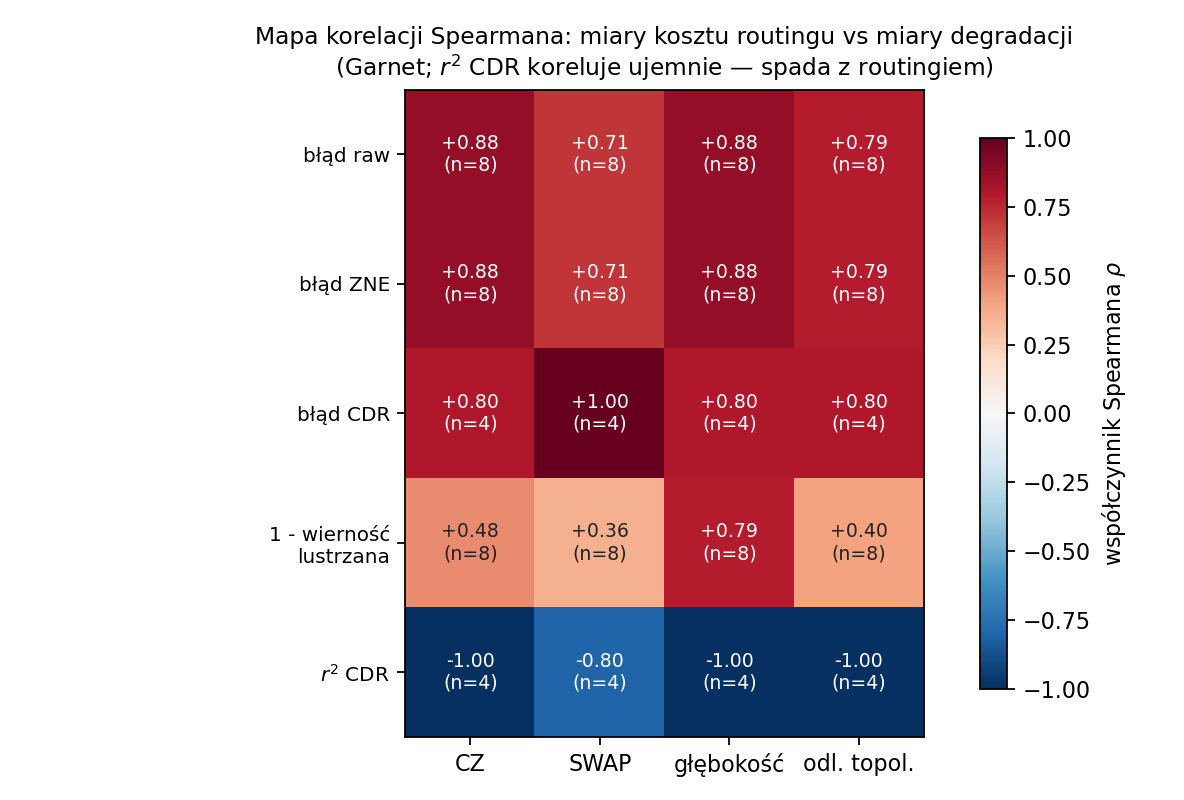
\includegraphics[width=0.72\textwidth]{fig5_correlation_map.png}
  \caption{Mapa korelacji rangowej Spearmana między miarami kosztu routingu a~miarami degradacji
  (Garnet). Liczba punktów podana w~każdej komórce; wiersze CDR opierają się na czterech punktach
  drabiny.}
  \label{fig:korelacje}
\end{figure}

Pełna mapa korelacji (Rysunek~\ref{fig:korelacje}) ujawnia trzy zależności wykraczające poza sam
wybór osi. Po pierwsze, \textbf{ZNE nie zmienia uporządkowania konfiguracji}: korelacje rangowe
błędu po ZNE są identyczne jak dla błędu bez mitygacji (kolejno $+0{,}88$, $+0{,}71$, $+0{,}88$,
$+0{,}79$). Mitygacja przeskalowuje wartości, ale nie odwraca hierarchii narzutu routingu -- złe
rozmieszczenie pozostaje złe. Po drugie, \textbf{błąd CDR koreluje z~liczbą bramek SWAP silniej
($+1{,}00$) niż z~samą liczbą CZ ($+0{,}80$)}, co jest spójne z~obrazem, w~którym to właśnie
łańcuchy SWAP wprowadzone przez router -- a~nie bramki dwukubitowe obwodu logicznego -- odpowiadają
za kumulację błędu koherentnego łamiącego dopasowanie. Po trzecie, \textbf{mirror fidelity
koreluje najsilniej z~głębokością ($+0{,}79$), a~słabo z~liczbą CZ ($+0{,}48$)}, podczas gdy błąd
klasyfikatora zachowuje się odwrotnie. Sugeruje to \emph{dwa różne kanały degradacji}: miara
niezależna od zadania jest wrażliwa przede wszystkim na czas trwania obwodu (dekoherencja), podczas
gdy metryka zadaniowa -- na liczbę operacji dwukubitowych. 

\paragraph{Miara niezależna od zadania.} Aby wyniki nie zależały wyłącznie od konkretnego
klasyfikatora, zmierzono na Garnecie \emph{mirror fidelity} -- obwód złożony ze swoją
odwrotnością, dla którego wynikiem idealnym jest powrót do stanu początkowego, a~zmierzona
przeżywalność stanowi czystą miarę jakości sprzętu, niezależną od zadania. Przeżywalność spada
z~$0{,}776$ przy 24~CZ do $0{,}215$--$0{,}277$ przy 66--150~CZ.

Ciekawsze od samego spadku jest to, \emph{z~czym} mirror infidelity koreluje, a~z~czym nie.
Zestawienie na wspólnych ośmiu punktach drabiny (Tabela~\ref{tab:mirror}) daje obraz jednoznaczny.

\begin{table}[h]\centering
\caption{Korelacje rangowe mirror infidelity z~pozostałymi wielkościami, na ośmiu wspólnych
punktach drabiny Garneta. Gwiazdka oznacza $p<0{,}05$.}
\label{tab:mirror}
\begin{tabular}{lcc}
\toprule
Mirror infidelity wobec & Spearman $\rho$ & $p$ \\
\midrule
głębokość obwodu po transpilacji & $+0{,}79^{*}$ & 0{,}021 \\
błąd klasyfikatora $\varepsilon$ & $+0{,}71^{*}$ & 0{,}047 \\
liczba bramek CZ & $+0{,}48$ & 0{,}233 \\
sumaryczna odległość topologiczna & $+0{,}40$ & 0{,}320 \\
liczba bramek SWAP & $+0{,}36$ & 0{,}385 \\
\midrule
\emph{względny zysk z~ZNE} & $-0{,}36$ & 0{,}385 \\
\bottomrule
\end{tabular}
\end{table}

Wyłaniają się z~tego dwa wnioski, z~których żaden nie jest trywialny.

\emph{Po pierwsze, mirror fidelity mierzy inną oś niż liczba bramek.} Koreluje najsilniej
z~\textbf{głębokością} obwodu ($+0{,}79$), a~z~liczbą bramek CZ już nieistotnie ($+0{,}48$). Jest to
spójne z~jej konstrukcją: obwód mirror jest dwukrotnie dłuższy w~czasie, więc dominuje w~nim
dekoherencja narastająca z~\emph{czasem trwania}, podczas gdy narzut routingu jest wielkością
\emph{zliczaną}. Obie osie są skorelowane, ale nie są tym samym; liczba CZ okazuje się
lepszym predyktorem błędu klasyfikatora ($+0{,}88$ wobec $+0{,}71$).

\emph{Po drugie mirror fidelity nie przewiduje, czy metoda mitygacji pomoże.}
Korelacja ze względnym zyskiem z~ZNE jest zerowa w~granicach błędu ($-0{,}36$, $p=0{,}39$; dla zysku
bezwzględnego $-0{,}07$). Widać to wprost w~danych: punkt \texttt{optimal:circular} ma najgorszą
mirror fidelity w~całym zbiorze ($0{,}215$), a~mimo to ZNE redukuje tam błąd o~$22\%$ --
więcej niż w~punkcie \texttt{optimal:linear}, którego przeżywalność jest ponad dwukrotnie lepsza
($0{,}527$), a~zysk wynosi zaledwie $2{,}7\%$.

\paragraph{Wniosek praktyczny: miara wierności mówi, jak źle jest, a~nie co pomoże.} Task-agnostyczny
wskaźnik jakości sprzętu odpowiada na pytanie ,,jak bardzo ten obwód jest zepsuty'', ale nie na
pytanie ,,która metoda to naprawi'' -- bo ta druga odpowiedź zależy od \emph{charakteru} szumu,
a~nie od jego wielkości. Wzmacnia to główną tezę metodologiczną pracy: żeby zdecydować o~wyborze
metody, trzeba zmierzyć jej własne założenie (dla CDR -- $r^2$), a~nie ogólny wskaźnik wierności.

\subsection{Mitygacja błędu odczytu na klasyfikatorze wariacyjnym}\label{sec:rem-wynik}

Zebrane dane pozwalają ocenić REM w~tym zastosowaniu, i~wynik jest jednoznacznie negatywny.
Uśredniając po 61 konfiguracjach (ansatz $\times$ głębokość $\times$ fold), REM redukuje
błąd $\varepsilon$ średnio o~$0{,}0017$, czyli o~\textbf{0{,}9\%} wartości,
\textbf{w~żadnej z~61 konfiguracji nie zmienia ani jednej decyzji klasyfikatora}: dokładność oraz
macro-F1 po REM są identyczne z~wartościami bez mitygacji we \emph{wszystkich} przypadkach.

Interpretacja jest prosta i~zgodna z~taksonomią z~Sekcji~\ref{sec:metody-mitygacji}: REM koryguje
wyłącznie ostatni etap obliczenia, podczas gdy stan wchodzący do pomiaru jest już zdegradowany przez
błędy bramkowe narosłe wzdłuż routingu. W~reżimie, w~którym pracujemy, błąd odczytu nie jest kanałem
dominującym. Uzasadnia to również decyzję o~wyłączeniu REM w~kampanii głównej -- niezależnie od
tego, że platforma IQM~Resonance nie udostępnia wymaganej kalibracji detektora.

\paragraph{Odzysk dokładności przy wysokim koszcie routingu.} W~dedykowanym pomiarze
o~podwyższonej statystyce (100 punktów ewaluacyjnych, 4096 pomiarów, 96~CZ) ZNE obniża błąd
$\varepsilon$ z~0{,}221 do 0{,}169 (o~24\%), lecz dokładność klasyfikacji pozostaje praktycznie
niezmieniona (0{,}78 wobec 0{,}77). Jest to istotny wynik negatywny dla zastosowań: w~reżimie
wysokiego narzutu routingu mitygacja poprawia metrykę ciągłą, ale \emph{nie odbudowuje} jakości
decyzji klasyfikatora -- poprawka nie wystarcza, by przesunąć punkty z~powrotem na właściwą stronę
granicy decyzyjnej.

% =====================================================================================
\section{Wnioski}\label{sec:wnioski}

Praca charakteryzuje reżimy opłacalności metod mitygacji błędów kwantowych jako funkcję narzutu
routingu, rozdzielone po topologiach, i~wskazuje mechanizm odpowiedzialny za obserwowane załamanie.

Po pierwsze, załamanie regresji danych Clifforda pod narzutem routingu jest \textbf{topologicznie
ogólne}: jakość dopasowania liniowego spada monotonicznie z~liczbą bramek dwukubitowych na każdej
badanej topologii, przy czym topologia gwiazdy wchodzi
w~region załamania przy blisko trzykrotnie niższym budżecie bramek niż krata ($\approx32$ wobec
$\approx86$~CZ). Teza opiera się na
trzech niezależnych pomiarach sprzętowych -- dwóch kratach o~różnym rozmiarze (Garnet 20q,
Emerald 54q) oraz jakościowo odmiennej topologii gwiazdy (ODRA 5q).

Po drugie, mechanizmem tego załamania jest błąd \textbf{koherentny}, naruszający założenie liniowości
CDR. Wskazuje na to symulacja towarzysząca: pod szumem niekoherentnym twirling nie daje zysku
i~nie wykazuje trendu, natomiast pod szumem koherentnym zysk jest dodatni, rośnie z~kosztem routingu
i~skaluje się z~amplitudą koherencji.

Po trzecie, \textbf{circuit twirling} przywraca skuteczność CDR na rzeczywistym sprzęcie. Zysk jest
istotny przy pośrednim koszcie routingu (57~CZ: $+0{,}069 \pm 0{,}023$, dodatni we wszystkich trzech
oknach kalibracyjnych) i~mieści się w~poziomie zerowym przy koszcie najniższym, gdzie koherencja nie
zdążyła się skumulować. Zależność od samej liczby bramek nie osiąga jednak istotności
($\rho=+0{,}32$, $p=0{,}41$), ponieważ przy najwyższym koszcie routingu dryf kalibracyjny dominuje
nad efektem. Właściwym predyktorem okazuje się \emph{stopień zniszczenia liniowości}: zysk twirlingu
koreluje z~jakością dopasowania bez twirlingu na poziomie $\rho=-0{,}85$ ($p=0{,}004$), przy czym
korelacja ta znacznie przekracza poziom generowany przez sprzężenie matematyczne w~danych
kontrolnych. \textbf{Twirling odzyskuje zatem tyle, ile koherencja wcześniej zepsuła}, a~liczba
bramek CZ jest jedynie zaszumionym pośrednikiem tej wielkości.

Po czwarte, granica opłacalności ZNE okazuje się \textbf{przewidywalna ilościowo}. Wyprowadzona
z~samej konstrukcji estymatora Richardsona stała $\kappa$ została potwierdzona pomiarem sprzętowym
dla \emph{dwóch} różnych zbiorów węzłów: $14{,}16 \pm 0{,}83$ wobec przewidywanych $14{,}656$ dla
$\{1,3,5\}$ ($0{,}60\sigma$) oraz $3{,}39 \pm 0{,}40$ wobec $4{,}000$ dla $\{1,3\}$ ($1{,}52\sigma$),
co daje wspólne nachylenie $0{,}937 \pm 0{,}049$ przy $\chi^2/\mathrm{dof} = 0{,}79$. Potwierdzeniu
podlega zatem nie pojedyncza liczba, lecz przewidziane $3{,}66$-krotne \emph{przeskalowanie} stałej
przy zmianie zbioru węzłów. Uzupełnia to niezależny test skalowania $S^{*}\propto B^{-2}$ (zgodność
10\%). Ponieważ $\kappa$ zależy wyłącznie od wyboru węzłów ekstrapolacji, liczba tych węzłów jest
\emph{decyzją projektową} przesuwającą próg opłacalności.

Zestawiając przewidywanie ,,pomoże czy zaszkodzi'' ze zmierzonym wynikiem we wszystkich
siedmiu punktach sprzętowych o~znanym $B$ i~$V$, granica $S^{*}=\kappa V/B^2$ trafia
w~\textbf{sześciu przypadkach na siedem}. Jedyna niezgodność -- Emerald przy 114~CZ -- nie jest
przy tym przypadkowa: należy do reżimu \emph{kolapsu sygnału}, czyli drugiego, niezależnie
zidentyfikowanego mechanizmu, wykrywanego osobną diagnostyką retencji. Złożenie obu reguł opisuje
wszystkie zmierzone punkty. Użytkownik dysponuje zatem kryterium, które można sprawdzić
\emph{przed} wydaniem czasu maszynowego, znając wyłącznie własny budżet pomiarów oraz zgrubne
oszacowanie obciążenia i~wariancji obserwabla.

Z~perspektywy praktycznej wyniki układają się w~regułę doboru metody. Poniżej około
\textbf{39~bramek CZ} korzystniejsze i~niemal siedmiokrotnie tańsze jest ZNE, pod warunkiem
że budżet pomiarów przekracza próg $S^{*}=\kappa V/B^2$; poniżej tego progu ZNE \emph{szkodzi}.
Powyżej punktu równowagi opłaca się CDR, którego zakres użyteczności rozszerza twirling. Powyżej
około \textbf{114~bramek CZ} żadna z~badanych metod nie przewyższa wyniku niemitygowanego. Wybór
rozmieszczenia kubitów, decydujący o~pozycji obwodu na tej osi, okazuje się przy tym decyzją równie
istotną co wybór samej metody mitygacji.

% =====================================================================================
\appendix
\section{Odtwarzalność: repozytorium}\label{sec:odtwarzalnosc}

Każda teza pracy daje się odtworzyć z~kodu i~danych zawartych w~repozytorium
(Tabela~\ref{tab:repo}). Flaga \texttt{--sim}
uruchamia identyczny potok na symulatorze (bezkosztowo), a~\texttt{--resume} pozwala dokończyć
przerwaną kampanię bez ponownego opłacania już zebranych punktów.

\begin{table}[h]\centering
\caption{Mapowanie: teza $\to$ skrypt $\to$ dane.}
\label{tab:repo}
\begin{tabular}{p{4.4cm}p{4.6cm}p{5.0cm}}
\toprule
Teza / wynik & Skrypt & Dane \\
\midrule
Drabina routingu, punkt wyjścia (ODRA) & \texttt{run\_hardware.py}, \texttt{zne\_dryrun.py} &
  \texttt{hardware\_results.csv}, \texttt{zne\_hard\_results.csv} \\
Kampania twirlingowa (3 okna) & \texttt{run\_garnet\_twirl.py} &
  \texttt{garnet\_twirl\_w\{1,2,3\}.csv} \\
Pasma dryfu, istotność, trend & \texttt{aggregate\_twirl\_windows.py} &
  \texttt{garnet\_twirl\_w123\_banded.csv} \\
Symulacja towarzysząca (null / koherencja) & \texttt{run\_garnet\_twirl.py --sim [--sim-coh]},
  \texttt{overnight\_sims.sh} & \texttt{night\_\{null,coh05,coh10\}\_banded.csv} \\
Koherencja na poziomie bramki & \texttt{run\_garnet\_urb.py} & wyniki w~Sek.~\ref{sec:mechanizm} \\
Cross-topology (Emerald) & \texttt{run\_garnet\_twirl.py --device emerald} &
  \texttt{emerald\_xtopo.csv} \\
Załamanie topologicznie ogólne & \texttt{analyze\_cross\_topology.py} &
  \texttt{cross\_topology\_summary.csv} \\
Progi metod & \texttt{analyze\_method\_threshold.py}, \texttt{analyze\_crossover.py} &
  \texttt{garnet\_crossover\_summary.csv} \\
Granica opłacalności ZNE & \texttt{zne\_boundary.py}, \texttt{zne\_shot\_boundary.py} &
  \texttt{zne\_shot\_boundary\_results.csv} \\
Test ogólności stałej $\kappa$ ($\{1,3\}$) & \texttt{zne\_shot\_boundary.py --scales 1 3} &
  \texttt{zne\_boundary\_k4\_results.csv} \\
Kampania ODRA (raw/CDR/ZNE) & \texttt{run\_odra\_cdr.py --zne} &
  \texttt{odra\_full\_100pt.csv} \\
Diagnostyka artefaktu ZNE & \texttt{zne\_signal\_retention.py} &
  \texttt{zne\_signal\_retention.csv} \\
Korelacje kosztu routingu & \texttt{analyze\_routing\_correlation.py} &
  \texttt{routing\_correlation\_summary.csv} \\
Mirror fidelity (miara task-agnostyczna) & \texttt{run\_garnet\_mirror.py} &
  \texttt{garnet\_mirror\_results.csv} \\
Rysunki & \texttt{make\_final\_figures.py} & \texttt{fig1--fig5\_*.png} \\
\bottomrule
\end{tabular}
\end{table}

\begin{thebibliography}{99}

\bibitem{cai2023}
Z. Cai, R. Babbush, S. C. Benjamin, S. Endo, W. J. Huggins, Y. Li, J. R. McClean,
T. E. O'Brien, \emph{Quantum Error Mitigation}, arXiv:2210.00921 (2023).

\bibitem{temme2017}
K. Temme, S. Bravyi, J. M. Gambetta, \emph{Error mitigation for short-depth quantum
circuits}, Phys. Rev. Lett. \textbf{119}, 180509 (2017); arXiv:1612.02058.

\bibitem{giurgica2020}
T. Giurgica-Tiron, Y. Hindy, R. LaRose, A. Mari, W. J. Zeng, \emph{Digital zero-noise
extrapolation for quantum error mitigation}, IEEE QCE (2020); arXiv:2005.10921.

\bibitem{kandala2019}
A. Kandala, K. Temme, A. D. Córcoles, A. Mezzacapo, J. M. Chow, J. M. Gambetta,
\emph{Error mitigation extends the computational reach of a noisy quantum processor},
Nature \textbf{567}, 491 (2019); arXiv:1805.04492.

\bibitem{czarnik2021}
P. Czarnik, A. Arrasmith, P. J. Coles, L. Cincio, \emph{Error mitigation with Clifford
quantum-circuit data}, Quantum \textbf{5}, 592 (2021); arXiv:2005.10189.

\bibitem{wallman2016}
J. J. Wallman, J. Emerson, \emph{Noise tailoring for scalable quantum computation
via randomized compiling}, Phys. Rev. A \textbf{94}, 052325 (2016); arXiv:1512.01098.

\bibitem{hashim2021}
A. Hashim i in., \emph{Randomized Compiling for Scalable Quantum Computing on a Noisy
Superconducting Quantum Processor}, Phys. Rev. X \textbf{11}, 041039 (2021); arXiv:2010.00215.

\bibitem{wallman2015}
J. J. Wallman, C. Granade, R. Harper, S. T. Flammia, \emph{Estimating the coherence of
noise}, New J. Phys. \textbf{17}, 113020 (2015); arXiv:1503.07865.

\bibitem{nielsen2010}
M. A. Nielsen, I. L. Chuang, \emph{Quantum Computation and Quantum Information},
Cambridge University Press (2010).

\bibitem{ferracin2022}
S. Ferracin i in., \emph{Efficiently improving the performance of noisy quantum computers}
-- synergetyczna mitygacja przez randomized compiling i ZNE, Quantum \textbf{8} (2024);
arXiv:2212.11198.

\bibitem{lowe2021}
A. Lowe, M. H. Gordon, P. Czarnik, A. Arrasmith, P. J. Coles, L. Cincio,
\emph{Unified approach to data-driven quantum error mitigation}, Phys. Rev. Research
\textbf{3}, 033098 (2021); arXiv:2011.01157.

\bibitem{mari2021}
A. Mari, N. Shammah, W. J. Zeng, \emph{Extending quantum probabilistic error cancellation
by noise scaling}, Phys. Rev. A \textbf{104}, 052607 (2021); arXiv:2108.02237.

\bibitem{vuillot2018}
C. Vuillot, \emph{Is error detection helpful on IBM 5Q chips?}, Quantum Inf. Comput.
\textbf{18}, 949 (2018); arXiv:1705.08957.

\bibitem{linke2017}
N. M. Linke i in., \emph{Fault-tolerant quantum error detection}, Sci. Adv. \textbf{3},
e1701074 (2017); arXiv:1611.06946.

\bibitem{li2019}
G. Li, Y. Ding, Y. Xie, \emph{Tackling the qubit mapping problem for NISQ-era quantum
devices (SABRE)}, ASPLOS (2019); arXiv:1809.02573.

\bibitem{schuld2021}
M. Schuld, R. Sweke, J. J. Meyer, \emph{The effect of data encoding on the expressive
power of variational quantum machine learning models}, Phys. Rev. A \textbf{103},
032430 (2021); arXiv:2008.08605.

\bibitem{perezsalinas2020}
A. Pérez-Salinas, A. Cervera-Lierta, E. Gil-Fuster, J. I. Latorre, \emph{Data re-uploading for
a universal quantum classifier}, Quantum \textbf{4}, 226 (2020); arXiv:1907.02085.

\bibitem{bowles2024}
J. Bowles, S. Ahmed, M. Schuld, \emph{Better than classical? The subtle art of
benchmarking quantum machine learning models}, arXiv:2403.07059 (2024).

% -- Artefakty, granice i warianty metod (przegląd literatury 2024--2026) --
\bibitem{koster2026}
M. Köster, W. Mauerer, \emph{Benchmarking Error Mitigation: Artefactual Improvements in
Zero-Noise Extrapolation}, arXiv:2607.09360 (2026).

\bibitem{alfaro2026}
V. Scavino Alfaro, \emph{The finite-shot help--harm boundary of zero-noise extrapolation},
arXiv:2605.08251 (2026).

\bibitem{quek2024}
Y. Quek, D. Stilck França, S. Khatri, J. J. Meyer, J. Eisert, \emph{Exponentially tighter
bounds on limitations of quantum error mitigation}, Nature Physics \textbf{20}, 1648 (2024);
arXiv:2210.11505.

\bibitem{sayapin2025}
Z. Sayapin, D. Rabinovich, N. Korolev, K. Lakhmanskiy, \emph{Zero-Noise Extrapolation via
Cyclic Permutations of Quantum Circuit Layouts}, arXiv:2511.02901 (2025).

\bibitem{googleqec2025}
Google Quantum AI and Collaborators, \emph{Quantum error correction below the surface code
threshold}, Nature \textbf{638}, 920--926 (2025).

\bibitem{maciejewski2020}
F.~B. Maciejewski, Z.~Zimborás, M.~Oszmaniec, \emph{Mitigation of readout noise in near-term
quantum devices by classical post-processing based on detector tomography},
Quantum \textbf{4}, 257 (2020).

\bibitem{nation2021}
P.~D. Nation, H.~Kang, N.~Sundaresan, J.~M. Gambetta, \emph{Scalable mitigation of measurement
errors on quantum computers}, PRX Quantum \textbf{2}, 040326 (2021).

\end{thebibliography}

\end{document}
